\documentclass[UTF8]{book}
\usepackage{ctex}
\usepackage[colorlinks=true]{hyperref}
\usepackage{amsmath}
\usepackage{amssymb}
\usepackage{tikz}
\usepackage{graphicx}
\usepackage{float}
\usepackage{geometry}
\usepackage{fancyhdr}
\usepackage{caption}
\usepackage{subcaption}
\usepackage[T1]{fontenc}
\usepackage{palatino}

\geometry{a4paper, left=2.5cm, top=2.5cm, bottom=2cm}
\geometry{hcentering}

\pagestyle{fancy}
\cfoot{\thepage}

\begin{document}
\title{深度学习笔记}
\author{zhliangqi}
\date{\today}

\maketitle

\tableofcontents

\chapter{Linear Algebra}

\section{特征值和特征空间}
\begin{equation}
    Au = \lambda u
\end{equation}
特征值$\lambda$代表线性变化的伸缩倍数,特征向量$u$代表变换的方向

\section{奇异值分解}
\textbf{定义} 对于$A \in C^{m \times n}$,$rank(A = r$,矩阵$A^HA$的特征值为
$\lambda_1 \geqslant \lambda_2 \geqslant ... \geqslant \lambda_r > 0$,
$\lambda_{r+1} = \lambda_{r+2} = ... = \lambda_{n} = 0$,称正数$\sigma_i = \sqrt{\lambda_i}(i = 1,2,...,r) $
为矩阵$A$的\textbf{奇异值}
\\
\begin{equation}
    \begin{split}
        A
        &= U \Sigma V^H \\
        &= (u_1\ u_2\ \cdot \cdot \cdot\ u_m)
        \begin{pmatrix}
            \lambda_1 &  &
        \end{pmatrix}
        \begin{pmatrix}
            v_1^H \\
            v_2^H \\
            \cdot \\
            \cdot \\
            \cdot \\
            v_n^H
        \end{pmatrix}
        \\
        &= \sigma_1 \boldsymbol{u}_1 \boldsymbol{v}_1^H + \sigma_2 \boldsymbol{u}_2 \boldsymbol{v}_1^H + \cdot\cdot\cdot + \sigma_r \boldsymbol{u}_r \boldsymbol{v}_r^H
    \end{split}
\end{equation}

\subsection{降维和图像压缩}
将图片作为矩阵进行奇异值分解,提取前n个奇异值,则可以达到图像压缩的目的.
\chapter{statistics}

\section{期望}
\section{方差}
均匀分布$X \sim R(a, b)$
其期望为
\begin{equation}
    \begin{split}
        E(X) &= \int_{a}^{b}x f(x) \mathrm{d}x		\\
        &= \frac{1}{b-a}\int_{a}^{b}x\mathrm{d}x	\\
        &= \frac{1}{b-a} \frac{1}{2} (b^2 - a^2)	\\
        &= \frac{1}{2}(b + a)
    \end{split}
\end{equation}
其方差为
\begin{equation}
    \begin{split}
        Var(X) &= E(X - EX)^2  \\
        &= E(X)^2 - (EX)^2 \\
        &= \int_{a}^{b} x^2 f(x) \mathrm{d}x - (EX)^2 \\
        &= \frac{1}{3(b-a)} (b^3 - a^3) - \frac{1}{4}(b+a)^2 \\
        &= \frac{1}{12}(b-a)^2
    \end{split}
\end{equation}
\\
对于正态分布$N(\mu, \sigma ^2)$,其期望$E(X) = \mu$,方差为$Var(X) = \sigma^2$.


\section{最小方差无偏估计}

\chapter{Basic}

\section{Mechine Learning}
\begin{itemize}
    \item supervised learning
    \item semi-supervised learning
    \item unsupervised learning
    \item reinforcement learning
    \item active learning
\end{itemize}

\section{iid}

\section{Universal approximation theorem}
\begin{quotation}
    Any continuous function can be uniformly approximated by a continuous neural network having only one
    internal, hidden layer and with an arbitrary continuous sigmoidal nonlinearity.\cite{Cybenko1989}
\end{quotation}
\par万能近似定理最初以sigmoidal激活函数来描述,后被证明对于更广泛的激活函数也适用\cite{Leshno1993},包括ReLU。

\section{Maximum likelihood estimation}
深度学习来就是用模型$p_{model}(\boldsymbol{x};\boldsymbol{\theta})$来估计数据的真实分布$p_{data}(\boldsymbol{x};\boldsymbol{\theta})$,对
于一组确定的数据集$X$,在样本已被观察到的情况下,需要找到使得$p_{model}(X; \boldsymbol{\theta})$出现可能性最大的一组参数$\boldsymbol{\theta}$,也就是
最大似然估计:
\begin{equation}
    \begin{split}
        \boldsymbol{\theta}_{ML} &= \arg \max_\theta p_{model}(X, \boldsymbol{\theta}) \\
        &= \arg \max_{\boldsymbol{\theta}} \prod _{i=1}^m p_{model}(\boldsymbol{x}^i; \boldsymbol{\theta})
    \end{split}
\end{equation}
等价于
\begin{equation}
    \begin{split}
        \boldsymbol{\theta}_{ML} &= \arg \max_{\boldsymbol{\theta}} \sum_{i=0}^m \log p_{model}(\boldsymbol{x}^i; \boldsymbol{\theta})
    \end{split}
\end{equation}
除$m$,等价于
\begin{equation}
    \begin{split}
        \boldsymbol{\theta}_{ML} &= \arg \max_{\boldsymbol{\theta}} E _{x \sim \hat p_{data}} \log p_{model}(\boldsymbol{x}^i; \boldsymbol{\theta})
    \end{split}
\end{equation}

\subsection{KL divergence}
KL散度用来衡量两种分布之间的差异,
\begin{equation}
    \begin{split}
        D_{KL}(\hat p_{data}|| p_{model}) &= \int_{-\infty}^{+\infty} \hat p_{data}(\boldsymbol{x}) \ln{\frac{\hat p_{data}(\boldsymbol{x})}{p_{model}(\boldsymbol{x})}} \mathrm{d}x
    \end{split}
\end{equation}
$\hat p_{data}(\boldsymbol{x})$与模型无关

\section{Initialization scheme}
\subsection{constant initialization}

\subsection{random initialization}
按照某一分布随机初始化
\subsubsection{normal initialization}
\begin{equation}
    W \sim N(\mu, \sigma^2)
\end{equation}

\subsubsection{uniform initalization}
\begin{equation}
    W \sim U[-\frac{1}{\sqrt{n}}, \frac{1}{\sqrt{n}}]
\end{equation}

\subsection{xavier initalization}
针对使用\textbf{对称激活函数}$\tanh(x)$的网络进行参数初始化,对于ReLU激活函数并不适用\cite{Glorot2010}.

\subsubsection{Forward}
对于一个卷积层来说
\begin{equation}
    \begin{split}
        \mathbf{y}_l &= \mathbf{W}_l \mathbf{x}_l + \mathbf{b}_l\\
        \mathbf{x}_l &= f(\mathbf{y}_{l-1})
    \end{split}
\end{equation}
在如下前提和假设下
\begin{itemize}
    \item 初始化$\mathbf{W}_l$元素为独立同分布
    \item 假设$\mathbf{x}_l$元素也为独立同分布
    \item $\mathbf{w}_l$, $\mathbf{x}_l$互相独立
\end{itemize}
则有
\begin{equation}
    \begin{split}
        Var(\mathbf{y}_l) &= Var(\sum \mathbf{w}_l \mathbf{x}_l + \mathbf{b}_l)\\
        &= Var(\sum \mathbf{w}_l \mathbf{x}_l) \\
        &= n_l Var(\mathbf{w}_l \mathbf{x}_l)
    \end{split}
\end{equation}
令$\mathbf{w}_l$期望为0,$E(\mathbf{w}_l) = 0, Var(\mathbf{w}_l) = E(\mathbf{w}_l - E(\mathbf{w}_l))^2 = E\mathbf{w}_l^2$,则
\begin{equation}
    \begin{split}
        Var(\mathbf{y}_l) &= n_l E(\mathbf{w}_l^2\mathbf{x}_l^2) - n_l E^2\mathbf{w}_l E^2 \mathbf{x}_l \\
        &= n_l E(\mathbf{w}_l^2\mathbf{x}_l^2) \\
        &= n_l Var(\mathbf{w}_l)E(\mathbf{x}_l^2)
    \end{split}
\end{equation}
若$E\mathbf{x}_l = 0$,则
\begin{equation}
    Var(\mathbf{y}_l) = n_l Var(\mathbf{w}_l)Var(\mathbf{x}_l)
\end{equation}

若要实现$Var(\mathbf{y}_l) = Var(\mathbf{x}_l)$,则需要满足$n_l Var(\mathbf{w}_l) = 1$,即
\begin{equation}
    Var(\mathbf{w}_l) = \frac{1}{n_l}
\end{equation}

\begin{itemize}
    \item 若$\mathbf{w}_l$服从正态分布,则$\mathbf{w}_l \sim N(0, \frac{1}{n_l})$
    \item 若$\mathbf{w}_l$服从均匀分布,则$\mathbf{w}_l \sim U(-\sqrt{\frac{3}{n_l}}, \sqrt{\frac{3}{n_l}})$
\end{itemize}

\subsubsection{Backword}
反向传播过程中,需要保证梯度的方差不变,每一层的梯度为:
\begin{equation}
    \Delta \mathbf{x}_l = \hat{\mathbf{W}}_l \Delta \mathbf{y}_l
\end{equation}
假设
\begin{itemize}
    \item $\mathbf{w}_l$和$\Delta{\mathbf{y}}_l$互相独立
    \item $E\mathbf{w}_l = 0, E\Delta{\mathbf{x}}_l = 0$
\end{itemize}
同前向传播,可得
\begin{equation}
    \begin{split}
        Var(\Delta{\mathbf{x}_l}) &= \hat n_l Var(\mathbf{w}_l)Var(\Delta{\mathbf{y}}_l)
    \end{split}
\end{equation}
\begin{itemize}
    \item 若$\mathbf{w}_l$服从正态分布, 则$\mathbf{w}_l \sim N(0, \frac{1}{\hat n_l})$
    \item 若$\mathbf{w}_l$服从均匀分布,则$\mathbf{w}_l \sim U(-\sqrt{\frac{3}{\hat n_l}}, \sqrt{\frac{3}{\hat n_l}})$
\end{itemize}

除非$n = \hat n_l$,否则同时保证信号在向前向后传播时的Var不变,取调和平均数,$Var(\mathbf{w}_l) = \frac{2}{n_l + \hat n_l}$,可得
\begin{itemize}
    \item Normal distribution: $\mathbf{w}_l \sim N(0, \frac{2}{n_l + \hat n_l})$
    \item Uniform distribution: $\mathbf{w}_l \sim U(-\sqrt{\frac{6}{n_l+\hat n_l}}, \sqrt{\frac{6}{n_l+\hat n_l}})$
\end{itemize}


\subsection{orthogonal initalization}

\subsection{kaiming initalization}
Xavier 针对对称激活函数的层权重初始化进行设计,但对于使用ReLu激活函数的层并不适用\cite{He2015}。
\par
对ReLU层来说,$E(\mathbf{x}_l^2) = \frac{1}{2}Var(\mathbf{y}_l)$,因此
\begin{equation}
    \begin{split}
        Var(\mathbf{y}_l) &= \frac{1}{2} n_l Var(\mathbf{w}_l)Var(\mathbf{x}_l) \\
        Var(\Delta{\mathbf{x}_l}) &= \frac{1}{2} \hat n_l Var(\mathbf{w}_l)Var(\Delta{\mathbf{y}}_l)
    \end{split}
\end{equation}
且在权重初始化时,使用上述任意一个即可。

\section{正则化}

\section{Data proprocessing}
\subsection{whitening}

\section{Activation functions}
\subsection{sigmoid}
\begin{tikzpicture}[domain=-2:2]
    \draw[very thin,color=gray] (-1.9, -1.9) grid (1.9, 1.9);
    \draw[->] (-2,0) -- (2,0) node[right] {$x$};
    \draw[->] (0,-2) -- (0,2) node[above] {$f(x)$};
    \draw[color=red]	plot (\x, { 1 / (1 + exp(-\x)) })   	node[right] {$g(x) = \frac{1}{1 + \mathrm{e^{-x}}}$};
\end{tikzpicture}

\begin{equation}
    \begin{split}
        g(x) &= \frac{1}{1+\mathrm{e}^{-x}} \\
        g(x)' &= g(x)(1-g(x))
    \end{split}
\end{equation}

\subsection{tanh(x)}
\begin{tikzpicture}[domain=-2:2]
    \draw[very thin,color=gray] (-1.9, -1.9) grid (1.9, 1.9);
    \draw[->] (-2,0) -- (2,0) node[right] {$x$};
    \draw[->] (0,-2) -- (0,2) node[above] {$f(x)$};
    \draw[color=blue]	plot (\x,{tanh(\x)})					node[right] {$g(x) = \tanh(x)$};
\end{tikzpicture}

\begin{equation}
    \begin{split}
        g(x) &= tanh(x) \\
        g(x)' &= 1 - g(x)^2 \\ &= 1 - \tanh(x)^2
    \end{split}
\end{equation}

\subsection{Rectified linear units}
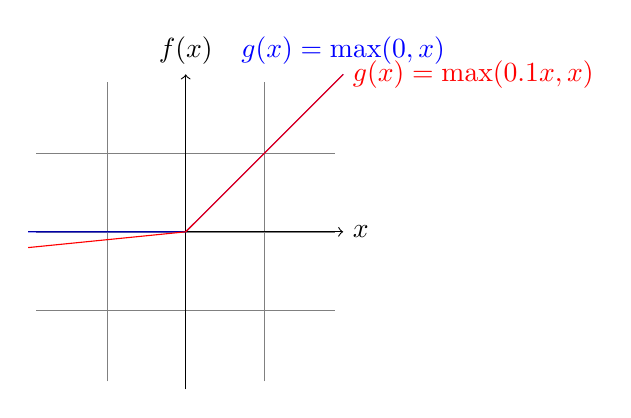
\begin{tikzpicture}[domain=-2:2]
    \draw[very thin,color=gray] (-1.9, -1.9) grid (1.9, 1.9);
    \draw[->] (-2,0) -- (2,0) node[right] {$x$};
    \draw[->] (0,-2) -- (0,2) node[above] {$f(x)$};
    \draw[color=blue]	plot (\x,{max(0, \x)})					node[above] {$g(x) = \max(0, x)$};
    \draw[color=red]	plot (\x,{max(0.1 * \x, \x)})			node[right] {$g(x) = \max(0.1x, x)$};
\end{tikzpicture}

\subsubsection{ReLU}
\begin{equation}
    g(x) = \max(0, x)
\end{equation}

\subsubsection{Leaky ReLU}
\begin{equation}
    g(x) = \max(0.01x, x)
\end{equation}

\subsubsection{PReLU}
\begin{equation}
    g(x) = \max(\alpha x, x)
\end{equation}

\subsection{haha}
\begin{tikzpicture}[domain=-2:2]
    \draw[very thin,color=gray] (-1.9, -1.9) grid (1.9, 1.9);
    \draw[->] (-2,0) -- (2,0) node[right] {$x$};
    \draw[->] (0,-2) -- (0,2) node[above] {$f(x)$};
    \draw[color=blue]	plot (\x,{tanh(\x) + 0.25 * \x})					node[right] {$g(x) = \tanh(x) + 0.25x$};
\end{tikzpicture}

\begin{equation}
    \begin{split}
        g(x) &= \tanh(x) + 0.25x \\
        g(x)' &= 0.75 - g(x)^2 \\ &= 0.75 - \tanh(x)^2
    \end{split}
\end{equation}

\subsection{Loss functions}



\section{信息熵}
\subsection{信息量}
信息量和具体的事件相关,且越小概率的事件发生产生的信息量越大。因此,\textbf{一个具体事件的信息量应该是随着其发生概率而递减的,且不能为负}。
如果我们有俩个不相关的事件x和y,那么我们观察到的俩个\textbf{独立事件同时发生时获得的信息应该等于观察到的事件各自发生时获得的信息之和},即为:
\begin{equation}
    \begin{split}
        h(x, y) &= h(x) + h(y) \\
        p(x, y) &= p(x) + p(y)
    \end{split}
\end{equation}
为满足以上性质,信息量$h(x)$公式为下
\begin{equation}
    h(x) = -\log_2p(x)
\end{equation}
\subsection{信息熵}
信息熵即为随机变量的信息量的期望
\begin{equation}
    H(x) = -\sum_ip(x_i)\log_2p(x_i)
\end{equation}
\subsection{条件熵}
\begin{equation}
    H(X|Y) = -\sum_{i,j}p(x_i, y_j)\log \frac{p(x_i, y_i)}{p(y_i)}
\end{equation}

\subsection{Mutual Information}
互信息是衡量随机变量之间互相依赖程度的度量。
\begin{equation}
    \begin{split}
        I(X;Y) &= H(X) - H(X|Y) \\
        &=\sum_y\sum_x p(x, y)\log(\frac{p(x, y)}{p(x)p(y)})
    \end{split}
\end{equation}

\section{Batch Normalization}
\begin{quotation}
    \textbf{Internal Covariate Shift} Training Deep Neural Networks is complicated by the fact that the distribution of each layer's inputs
changes during training, as the parameters of the previous layers change. And this slows down the training 
by requring lower lr ant careful parameter initialization, and makes it notoriously hard to train models
with saturating nonlinearities.
\end{quotation}
\begin{quotation}
    By whitening the inputs to each layer, we would take a step towards achieving the fixed distribution
    of inputs that would remove the ill effects of the ICS.
\end{quotation}
但是每层的白化会影响梯度下降优化过程。每层进行白化计算量过大。保证模型的表达能力不因为规范化而下降。
Simply normalizaing each input of a layer may change what the layer can represent. So, we make sure that
the transformation inserted in the network can represent the identity transform.
\chapter{Optimization Algorithms}
如果梯度只用来指示方向,大小完全由lr决定?
\section{Challenges}

\begin{figure}
    \centering
    \begin{minipage}[b]{0.32\textwidth}
        \centering
        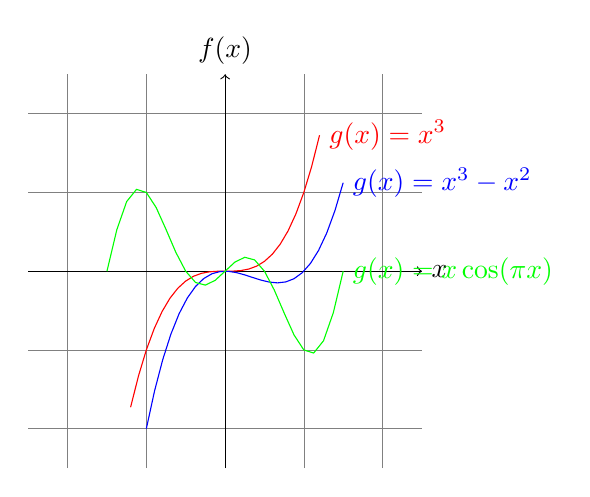
\begin{tikzpicture}
            \draw[very thin,color=gray] (-2.5, -2.5) grid (2.5, 2.5);
            \draw[->] (-2.5,0) -- (2.5,0) node[right] {$x$};
            \draw[->] (0,-2.5) -- (0,2.5) node[above] {$f(x)$};
            \draw[red,domain=-1.2:1.2]	plot (\x, { \x * \x * \x })   	node[right] {$g(x) = x^3 $};
            \draw[blue,domain=-1.0:1.5]	plot (\x, { \x * \x * \x - \x * \x })   	node[right] {$g(x) = x^3 - x^2$};
            \draw[green,domain=-1.5:1.5]	plot (\x, { \x * cos(3.1415926 * \x r) })   	node[right] {$g(x) = x\cos(\pi x) $};
        \end{tikzpicture}
    \end{minipage}
    \begin{minipage}[b]{0.32\textwidth}
        \centering
        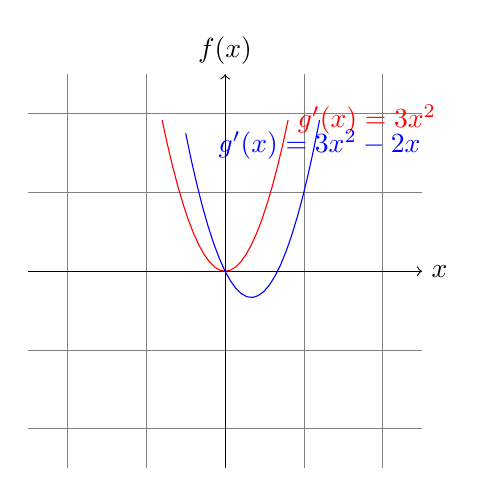
\begin{tikzpicture}
            \draw[very thin,color=gray] (-2.5, -2.5) grid (2.5, 2.5);
            \draw[->] (-2.5,0) -- (2.5,0) node[right] {$x$};
            \draw[->] (0,-2.5) -- (0,2.5) node[above] {$f(x)$};
            \draw[red,domain=-0.8:0.8]	plot (\x, { 3 * \x * \x })   	node[right] {$g'(x) = 3x^2 $};
            \draw[blue,domain=-0.5:1.2]	plot (\x, { 3 * \x * \x - 2 * \x})   	node[below] {$g'(x) = 3x^2 - 2x$};
        \end{tikzpicture}
    \end{minipage}
    \begin{minipage}[b]{0.32\textwidth}
        \centering
        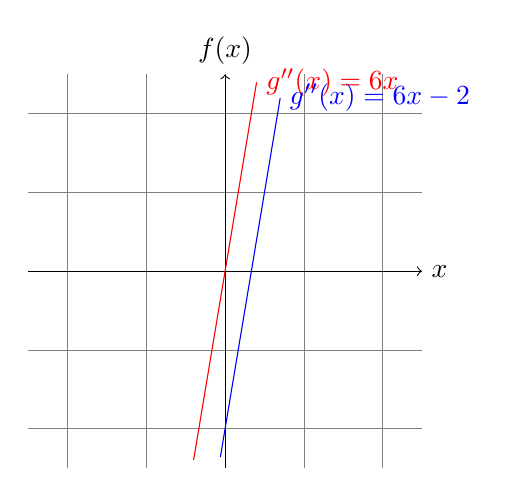
\begin{tikzpicture}
            \draw[very thin,color=gray] (-2.5, -2.5) grid (2.5, 2.5);
            \draw[->] (-2.5,0) -- (2.5,0) node[right] {$x$};
            \draw[->] (0,-2.5) -- (0,2.5) node[above] {$f(x)$};
            \draw[red,domain=-0.4:0.4]	plot (\x, { 6 * \x })   	node[right] {$g''(x) = 6x $};
            \draw[blue,domain=-0.06:0.7]	plot (\x, { 6 * \x - 2 })   	node[right] {$g''(x) = 6x - 2$};
        \end{tikzpicture}
    \end{minipage}
    \caption{Challenges}
\end{figure}


\subsection{Local Minima}
\begin{quotation}
    When the numerical solution of an optimization problem is near the local optimum, the numerical
    solution obtained by the final iteration may only minimize the objective function locally, rather
    than globally, as the gradient of the objective function's solutions approaches or becomes zero.
    \textit{Only some degree of noise might knock the parameter out of the local minimium. In fact,
        this is the one of the beneficial properties of stochastic gradient descent where the natural variation
        of gradients over minibatches is able to dislodge the parameters from loacl minima.}\cite{zhang2020dive}
\end{quotation}
\subsection{Saddle Points}
\begin{quotation}
    We assume that the input of a function is $k$-dimensional vector and its ouput is a scalar,
    so its \textit{Hession matrix} will have \textit{$k$ eigenvalues}. The solution of the function could
    be a local minimum, a local maximum or a saddle point at a position where the function gradient
    is zero:
    \begin{itemize}
        \item When the eigenvalues of the function's Hession matrix at the zero-gradient position 
        are all positive, we have a local minimum for the function.
        \item When the eigenvalues of the function's Hession matrix at the zero-gradient position 
        are all negative, we have a local maximum for the function.
        \item When the eigenvalues of the function's Hession matrix at the zero-gradient position 
        are negative and positive, we have a saddle point for the function.
        \item 同号且至少有一个为0,不确定
    \end{itemize}
    For high-dimensional problem the likehood that at least some of the eigenvalues are negative
    is quite high. This makes sadlle points are more likely then local minima.\cite{zhang2020dive}
\end{quotation}

\subsection{Vanishing gradients}
\begin{quotation}
    Vanishing gradients can cause optimization to stall. Often a reparameterization of the problem
     helps. Good initialization of the parameters can be beneficial, too.\cite{zhang2020dive}
\end{quotation}

\subsection{Gradient Descent}
Using a Taylor expansion we obtain that:
\begin{equation}
    f(x + \epsilon) = f(x) + \epsilon f'(x) + \mathcal{O} (\epsilon^2)
\end{equation}
\par
For small $\epsilon$ moving in \textit{the direction of negative gradient} will decrease $f$. Choose $\epsilon = 
-\eta f'(x), \eta > 0$, then we get:
\begin{equation}
    f(x - \eta f'(x)) = f(x) - \eta f'^2(x) + \mathcal{O} ((\eta f'(x))^2)
\end{equation}
\par Choose $\eta$ samll enough for the higher order terms to become irrelevant. then
\begin{equation}
    f(x - \eta f'(x)) \lessapprox f(x)
\end{equation}
that means, if we use 
\begin{equation}
    x \leftarrow x - \eta f'(x)
\end{equation}
to iterate x, the value of $f(x)$ decline.

\subsection{Adaptive Methods}
Getting the learning rate 'just right' is tricky. What if we could determine $\eta$ automatically or get rid of having to select
a setp size at all? Second order methods that look not only at the value and gradient of the objective but alse at its \textit{curvature}
can help in this case. These methods cannot be applied to deep learning directly due to the computational cost.

\subsubsection{Newton's Method}
当Taylor expansion展开到二阶导数时:
\begin{equation}
    f(\mathbf{x} + \epsilon) = f(\mathbf{x}) + \epsilon^\top \nabla f(\mathbf{x}) + \frac{1}{2} \epsilon^\top H_f \epsilon 
    + \mathcal{O}(\|\epsilon\|^3)
\end{equation}
we define $H_f := \nabla \nabla ^\top f(\mathbf{x})$ to be the \textit{Hession} of $f$. $H$ is a $d \times  d$ matrix and may be
prohibitively large, due to the cost of storing $\mathcal{O}(d^2)$ entries.

\par

After all, the minimum of $f$ statifies $\nabla f(\mathbf{x}) = 0$.  Taking derivatives of above equtaion with regard to $\eta$ and 
ignoring higher order terms we arrive at 
\begin{equation}
   \begin{split}
    \nabla f(\mathbf{x}) + H_f \epsilon = 0 \\
    \mathbf{\epsilon} = -H_f^{-1} \nabla f(\mathbf{x})
   \end{split}
\end{equation}

then, $\epsilon = -\eta \nabla f(\mathbf{x})$, we get
\begin{equation}
    \begin{split}
        \mathbf{\eta} = -H_f^{-1}
    \end{split}
\end{equation}

For $f(x) = (x-2)(x-4) = x^2 - 6x + 8, f'(x) = 2x - 6, f''(x) = 2$, then
\begin{equation}
    \epsilon = -f''(0)^{-1} f'(0) = -\frac{1}{2} \times -6 = 3 
\end{equation}

\subsubsection{Hessian}
Hession 矩阵是是对称的,可以表示为一组特征值和一组特征向量的正交基底,在特定方向上$g$上的二阶导数为$g^\top H g$,当$g$为特征向量时,这个二阶导数就是
对应的特征值。最大特征值确定最大二阶导数,最小特征值确定最小导数。\par
在$g$方向上的learning rate为
\begin{equation}
    \eta_g = \frac{1}{g^\top H_f g}
\end{equation}
最差的情况下,$g$与$H$最大的特征值$\lambda_{max}$对应的特征向量对齐,此时的最优步长为$\frac{1}{\lambda_{max}}$,当要最小化的目标函数能用二次函数
很好近似的情况下,Hession的特征值决定了学习率的量级。

\subsection{Stochastic Gradient Descent}
\subsubsection{Dynamic Learning rate}

\begin{equation}
    \begin{aligned}
        \eta(t) &= \eta_i \text{ if } t_i \leq  t \leq t_{i+1} & & piecewise constant\\
        \eta(t) &= \eta_0 e^{-\lambda t} & & exponential\\
        \eta(t) &= \eta_0 (\beta t + 1) ^{-\alpha} && polynomial
    \end{aligned}
\end{equation}
In the case of convex optimization there are a number of proofs which show that this rate is well behaved.

\subsection{Minibatch Stochastic Gradient Descent}
\chapter{Models}
\section{LeNet-5}
\begin{figure}[H]
    \centering
    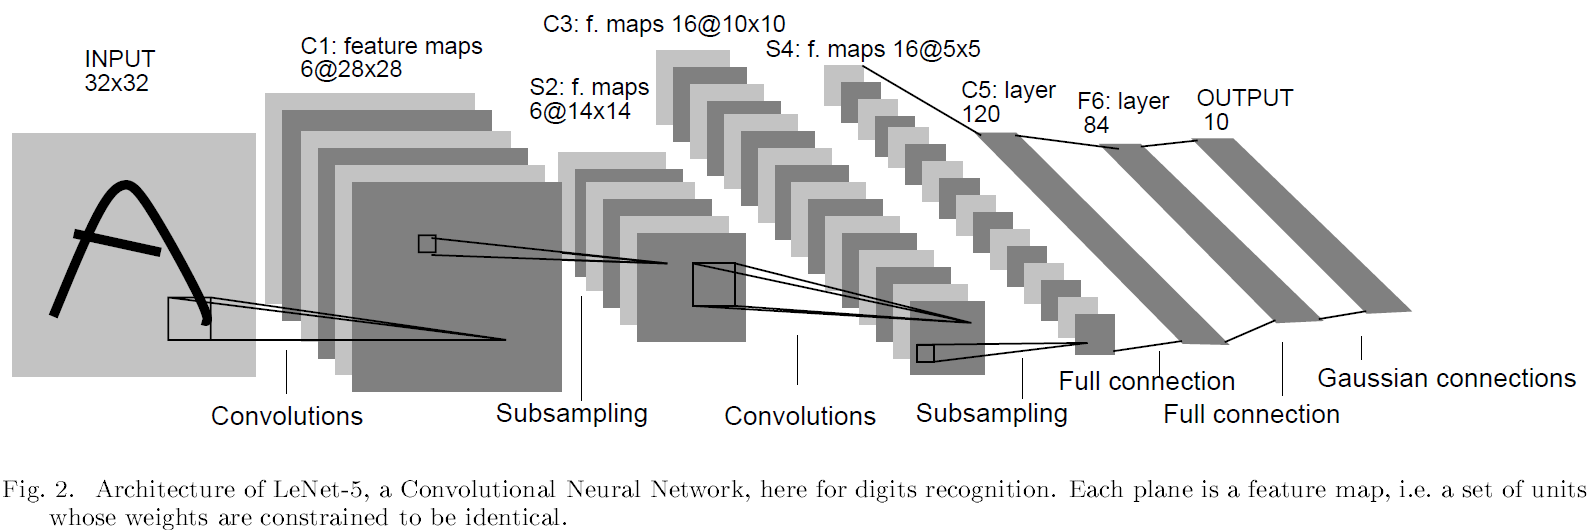
\includegraphics[width=16cm]{images/models/lenet-5.png}
    \label{fig:lenet-5}
\end{figure}

\section{AlexNet}
\begin{figure}[H]
    \centering
    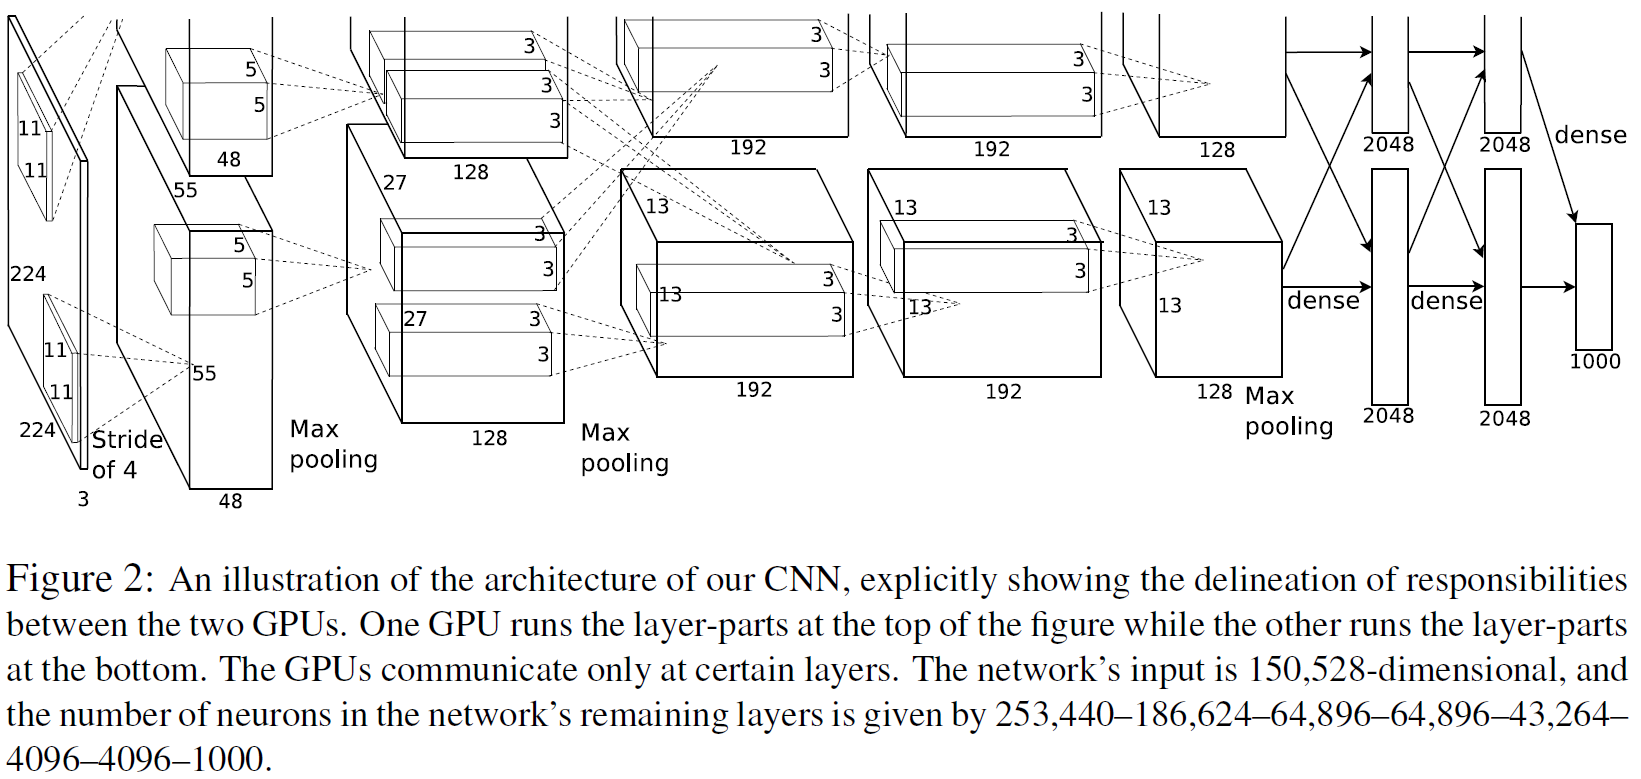
\includegraphics[width=16cm]{images/models/alexnet.png}
    \label{fig:alexnet}
\end{figure}

\section{VGG}
\begin{figure}[H]
    \centering
    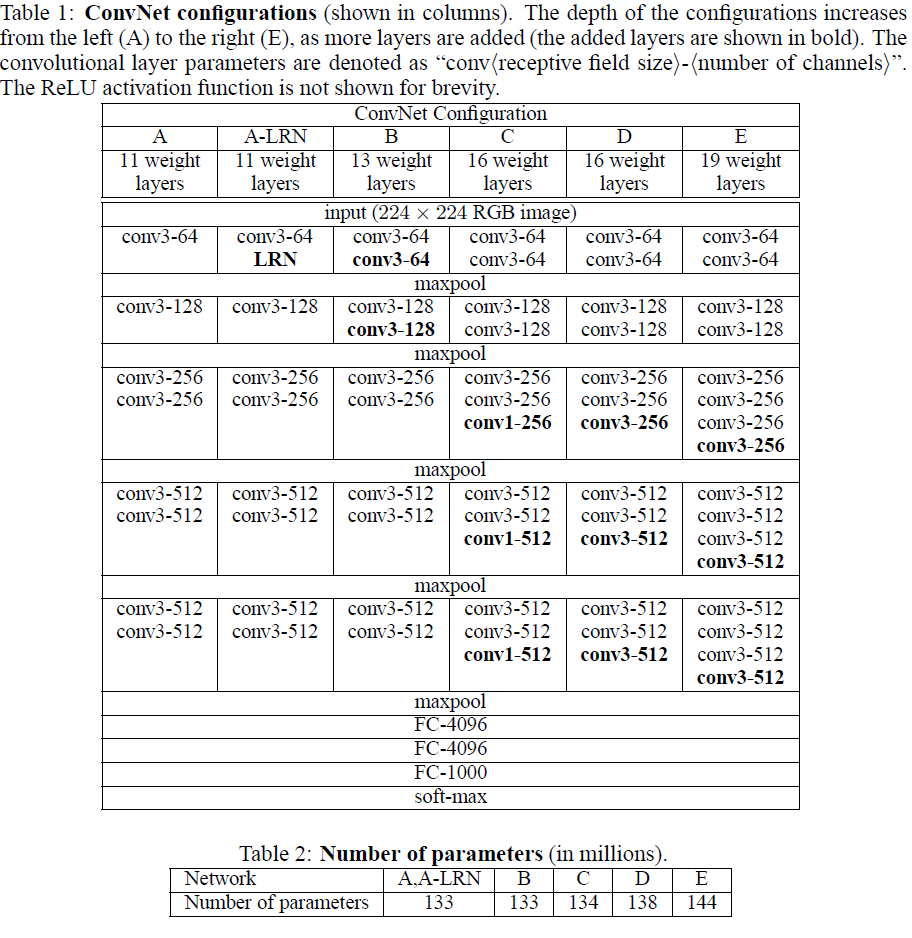
\includegraphics[width=16cm]{images/models/vgg.png}
    \label{fig:vgg}
\end{figure}

\section{GoogLeNet(Inception-v1)}
\subsection{Inception Module}
\begin{figure}[H]
    \centering
    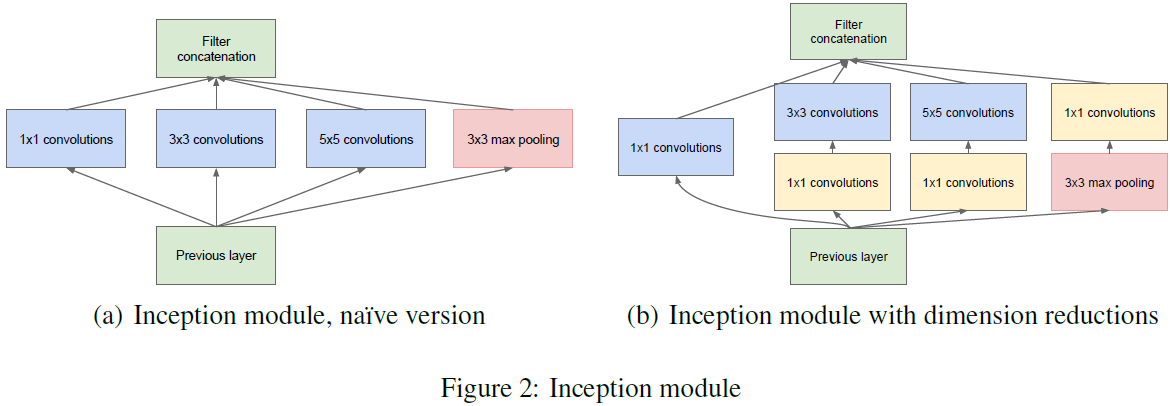
\includegraphics[width=14cm]{images/models/inception_module.png}
    \label{fig:inception_module}
\end{figure}

\subsection{Inception-v1}

\begin{figure}[H]
    \centering
    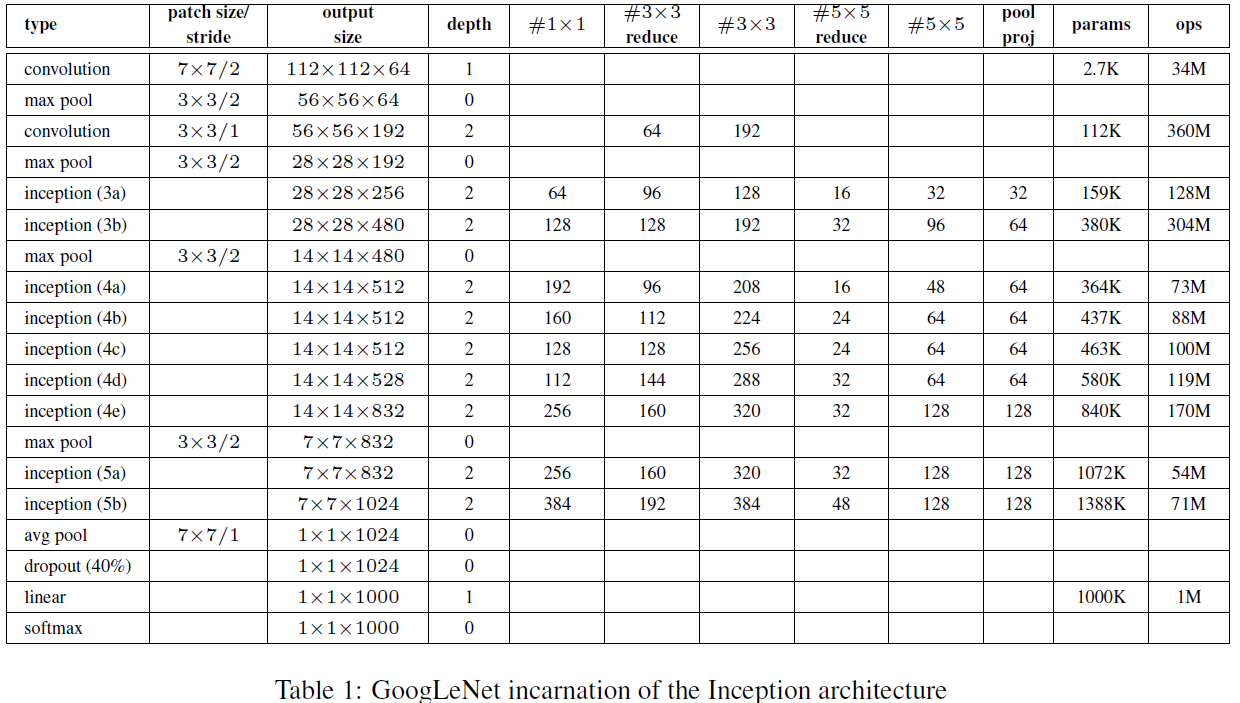
\includegraphics[width=16cm]{images/models/googlenet.png}
    \label{fig:googlenet}
\end{figure}

\begin{figure}[H]
    \centering
    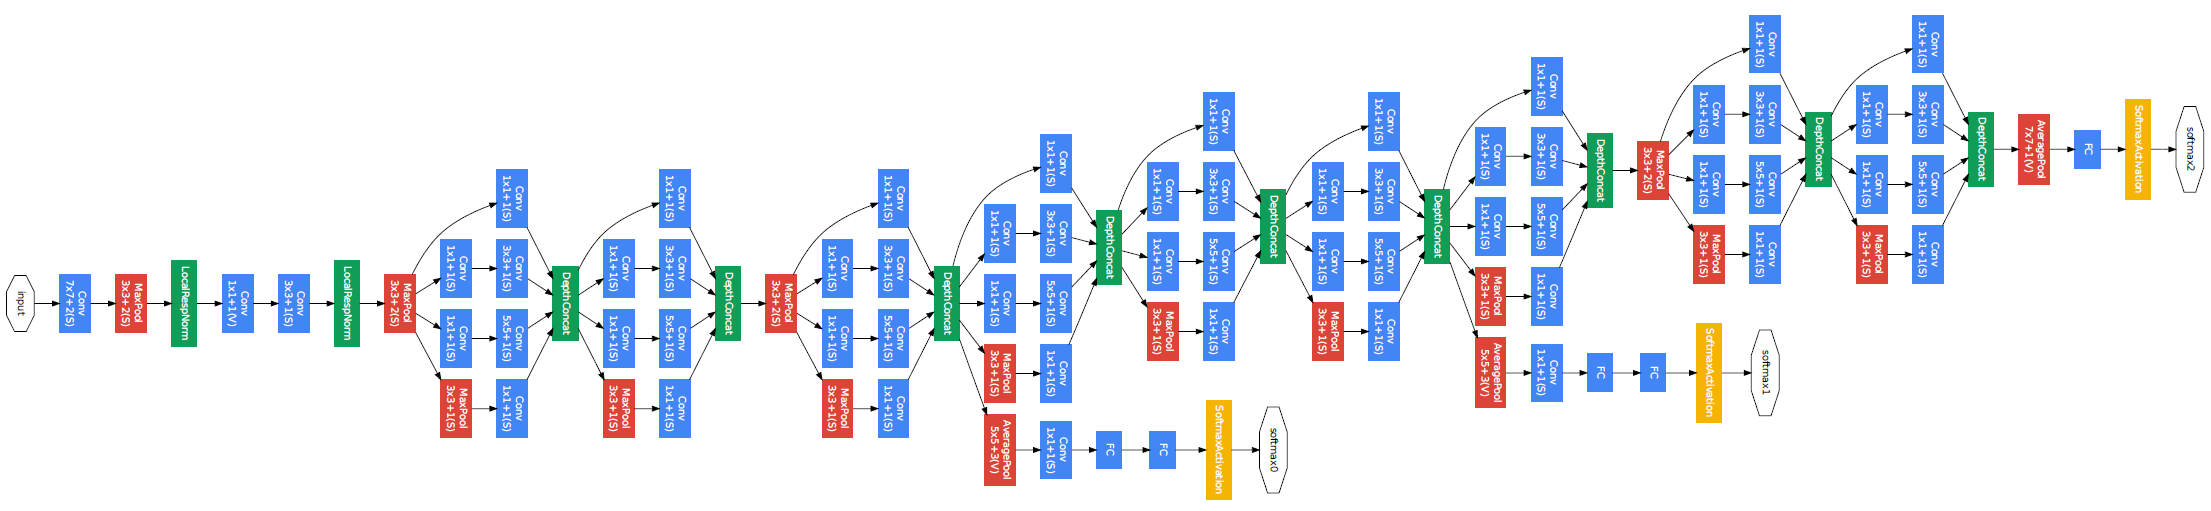
\includegraphics[width=16cm]{images/models/googlenet_arch.png}
    \label{fig:googlenet_arch}
\end{figure}

\section{ResNets}
\subsection{Residual Block}
\begin{figure}[H]
    \centering
    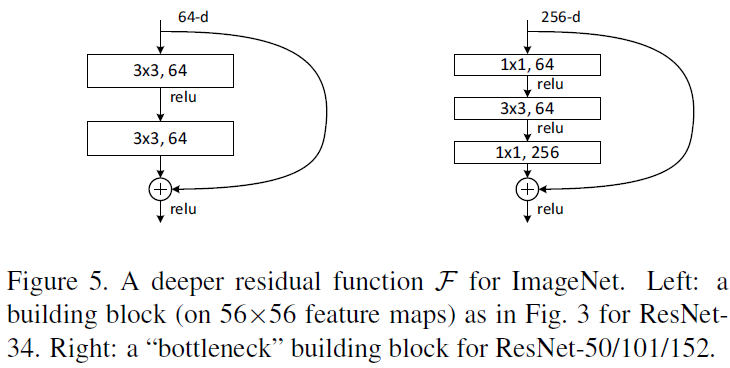
\includegraphics[width=8cm]{images/models/residualblock.png}
    \label{fig:residualblock}
\end{figure}

\subsection{ResNets}
\begin{figure}[H]
    \centering
    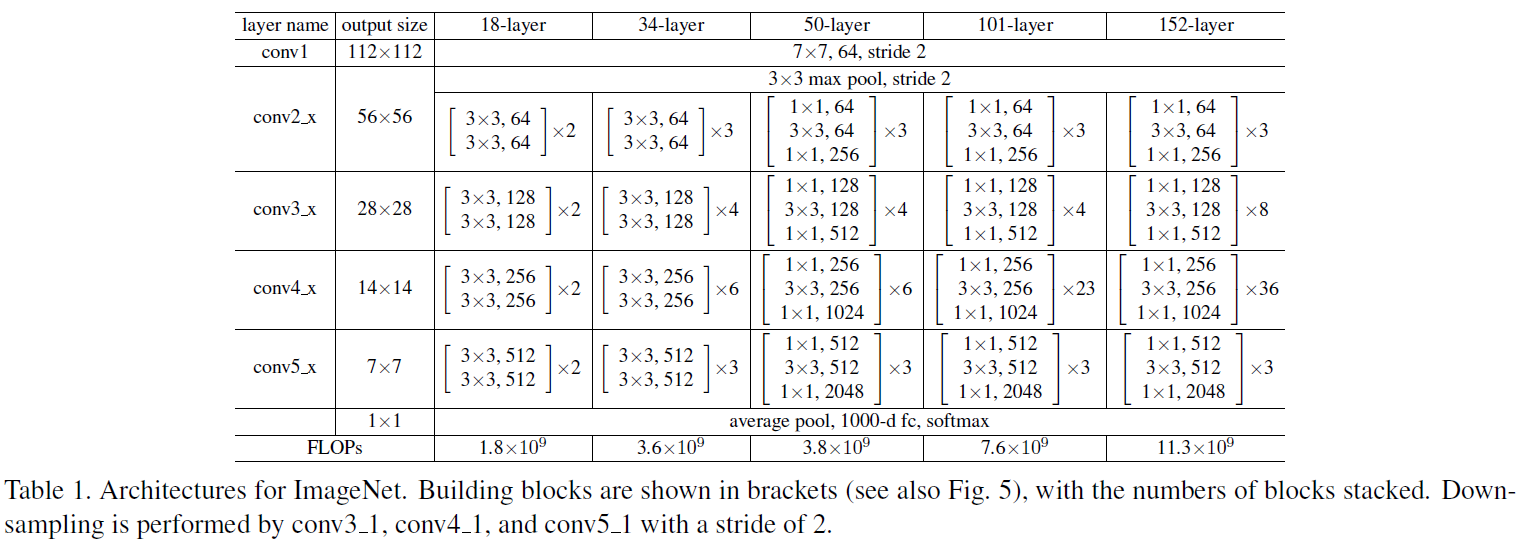
\includegraphics[width=16cm]{images/models/resnets.png}
    \label{fig:resnets}
\end{figure}
\begin{figure}[H]
    \centering
    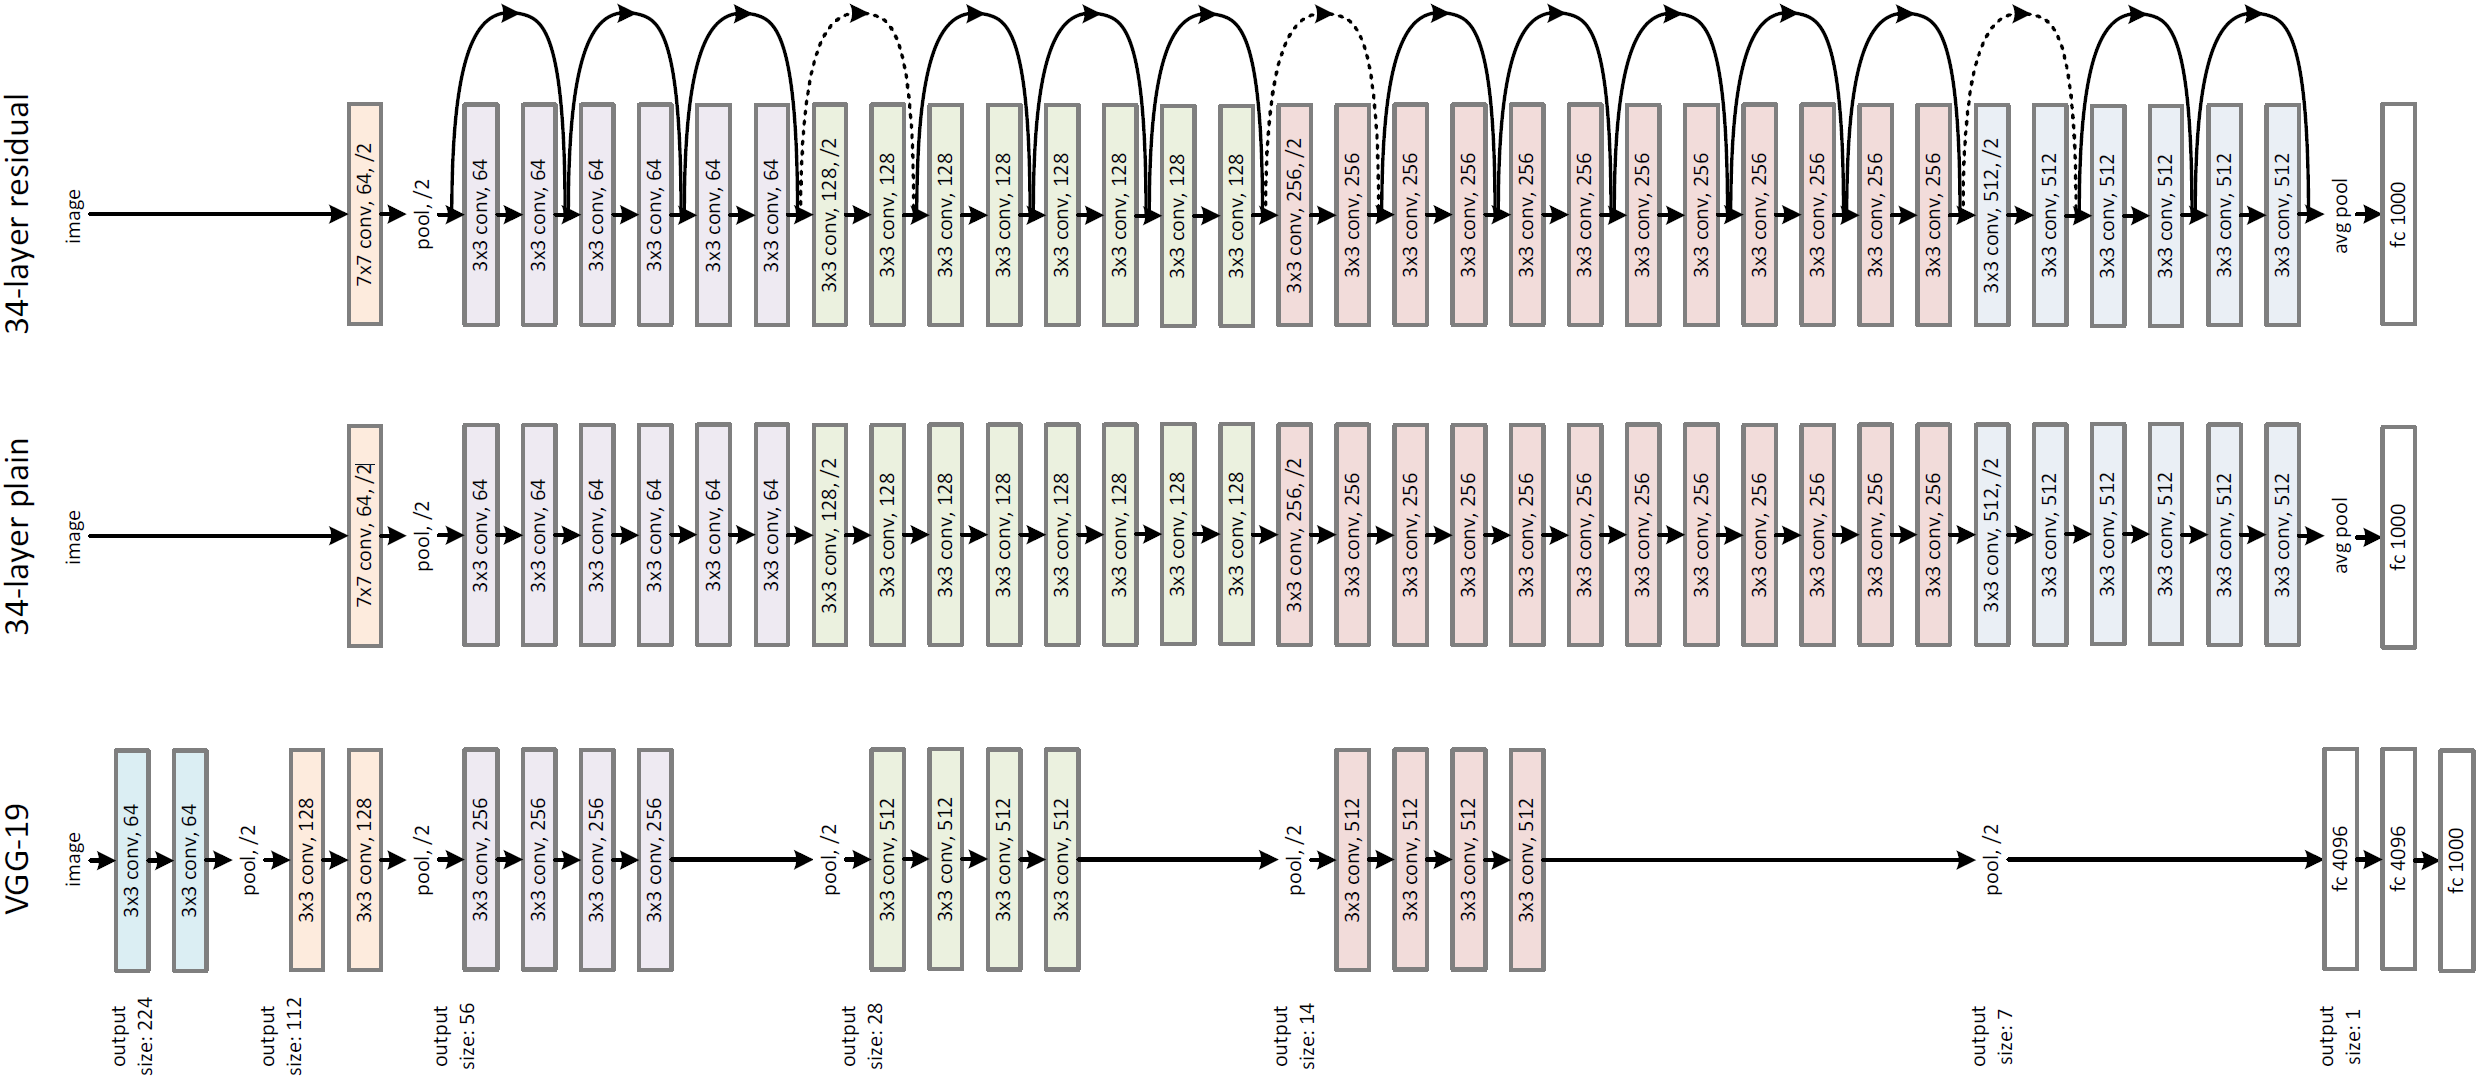
\includegraphics[width=16cm]{images/models/resnets_arch.png}
    \label{fig:resnets_arch}
\end{figure}

\section{Inception-v2, Inception-v3}
\subsection{General Design Principles}
\begin{itemize}
    \item Avoid representational bottlenecks, especially early in the network.
    \item Higher dimensional representations are easier to process locally within a network.
    \item Spatial aggregation can be done over lower dimensional embeddings without much or any loss in representational power.
    \item Balance the width and depth of the network.
\end{itemize}

\subsection{Inception Modules}

\begin{figure}[htbp]
    \centering

    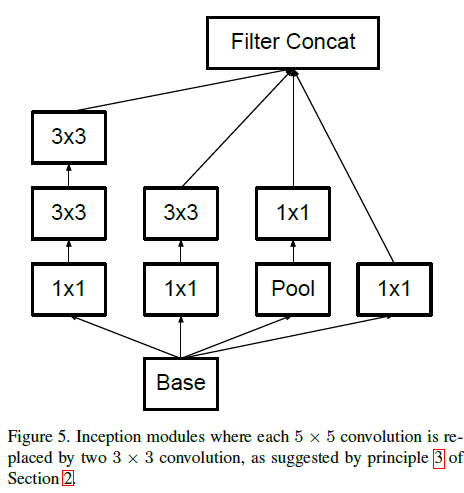
\includegraphics[width=6cm]{images/models/inception_m1.png}
    \hspace{1in}
    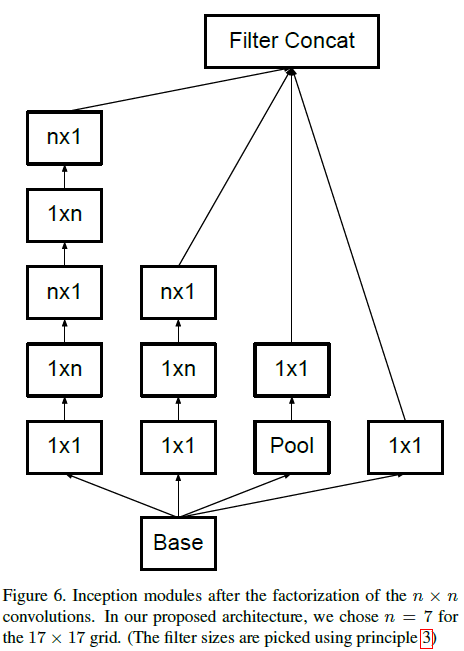
\includegraphics[width=6cm]{images/models/inception_m2.png}
    \hspace{1in}
    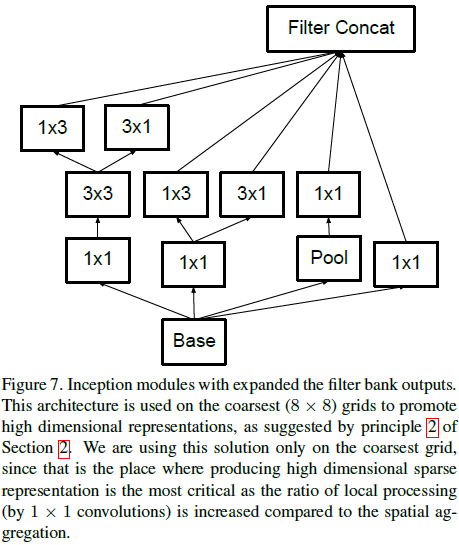
\includegraphics[width=6cm]{images/models/inception_m3.png}
    \hspace{1in}
    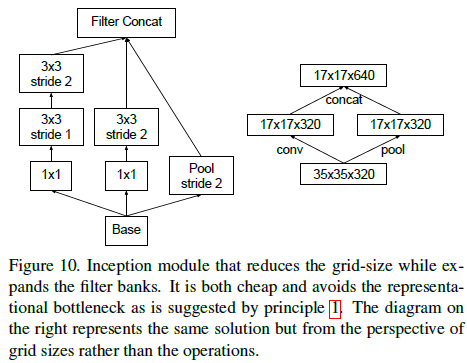
\includegraphics[width=6cm]{images/models/inception_m4.png}
    \caption{Inception Modules}
\end{figure}

\subsection{Inception-v2}
\begin{figure}[H]
    \centering
    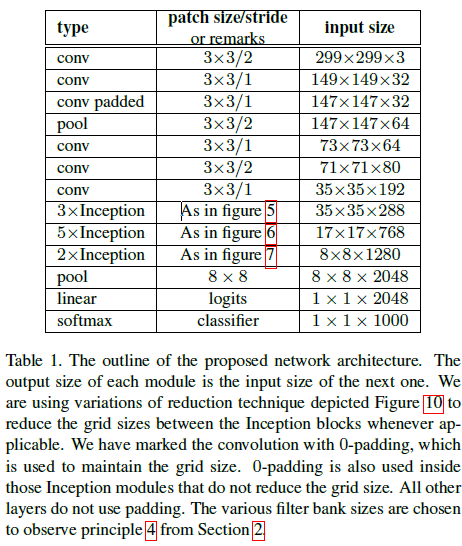
\includegraphics[width=8cm]{images/models/inception_v2v3.png}
    \label{fig:inception_v2v3}
\end{figure}

\subsection{Inception-v3}
\begin{itemize}
    \item RMSProp Optimizer.
    \item Factorized 7x7 convolutions.
    \item BatchNorm in the Auxillary Classifiers.
    \item Label Smoothing
\end{itemize}

\section{Inception-v4, Inception-ResNet}

\section{Xception}
\begin{quotation}
    We present an interpretation of Inception modules 
as being an intermediate step in-between regular convolution
and the depthwise separable convolution operation. In this
light, a depthwise separable convolution can be understood
as an Inception module with a maximally large number of towers.
\end{quotation}

\subsection{Xception Module}
\begin{figure}[H]
    \centering
    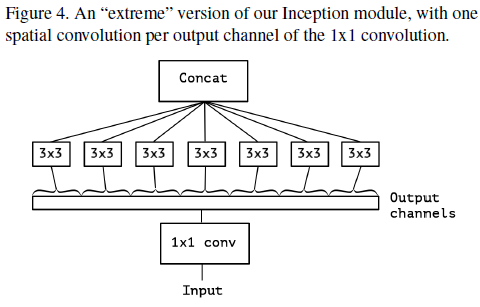
\includegraphics[width=8cm]{images/models/xception_m.png}
    \label{fig:xception_m}
\end{figure}

\subsection{Xception}
\begin{figure}[H]
    \centering
    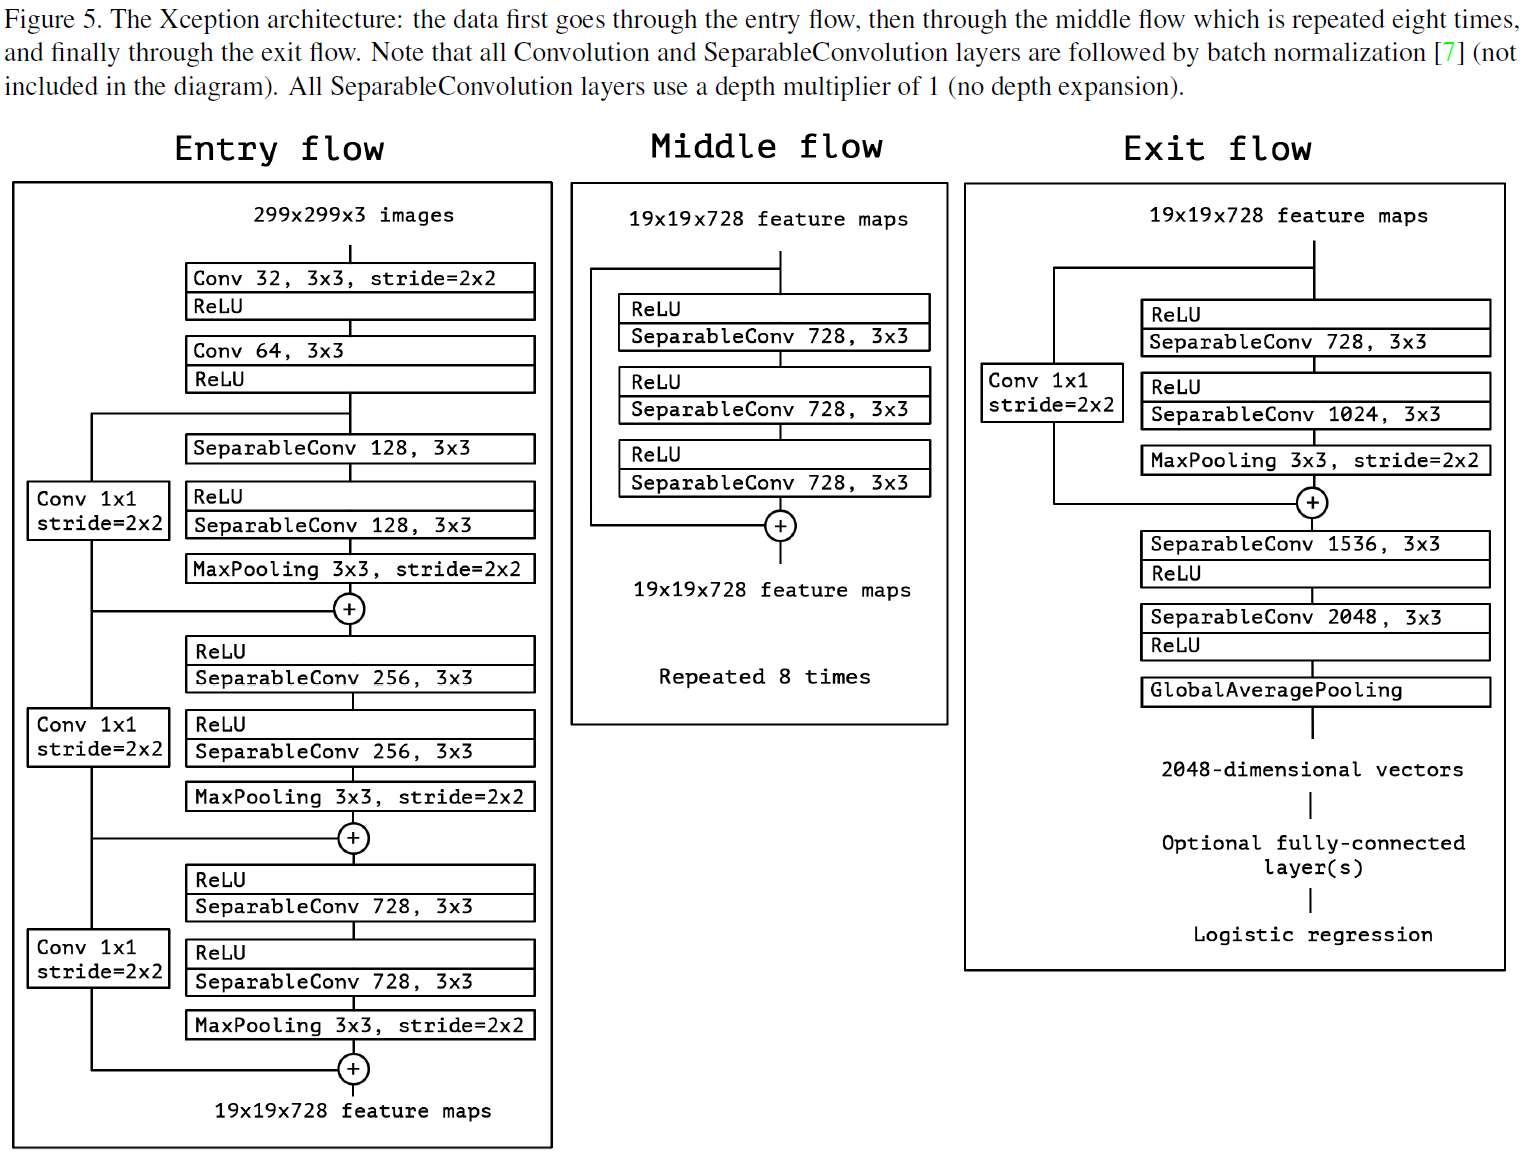
\includegraphics[width=16cm]{images/models/xception.png}
    \label{fig:xception}
\end{figure}

\section{ResNeXt}
Group Convolution + Skip connection

\subsection{ResNeXt Block}
\begin{figure}[H]
    \centering
    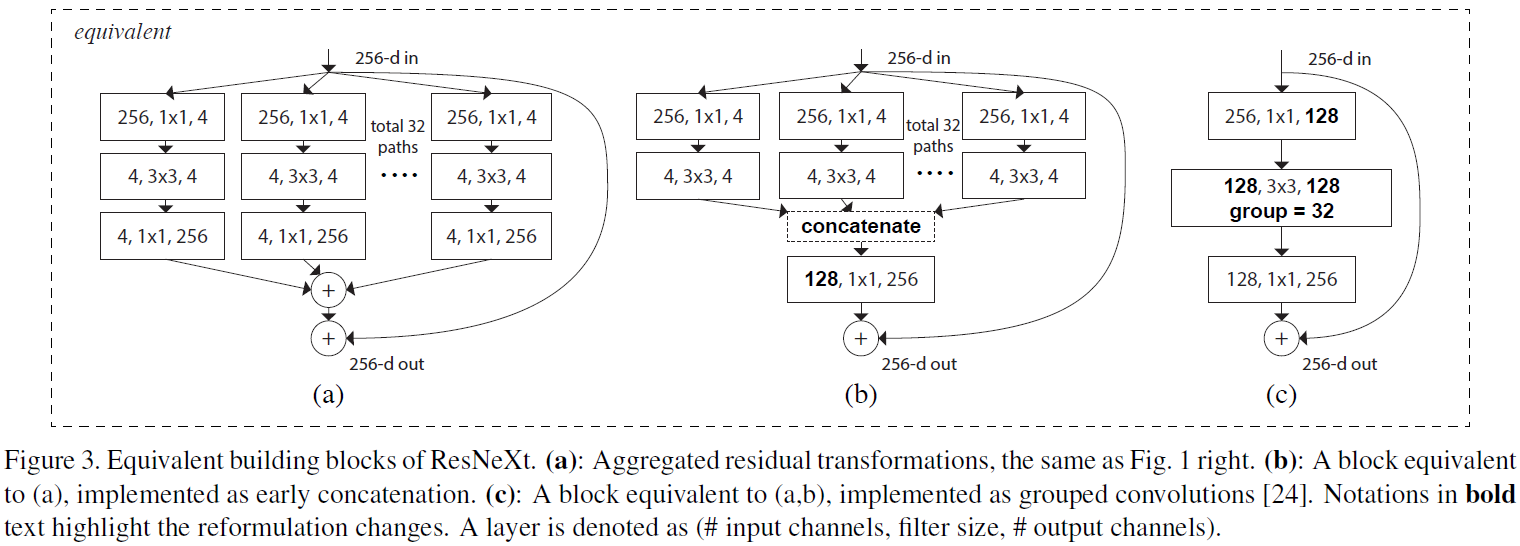
\includegraphics[width=16cm]{images/models/resnext_blocks.png}
    \label{fig:resnext_blocks}
\end{figure}

\subsection{ResNeXt}
\begin{figure}[H]
    \centering
    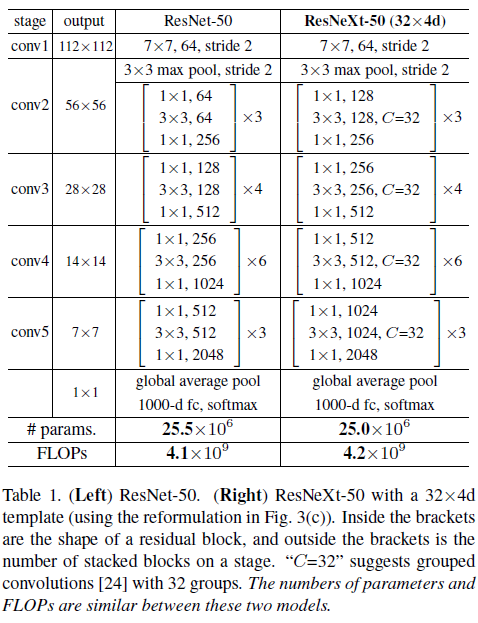
\includegraphics[width=8cm]{images/models/resnext.png}
    \label{fig:resnext}
\end{figure}

\section{MobileNets}

\subsection{Depthwise Separable Convolution}
\begin{figure}[H]
    \centering
    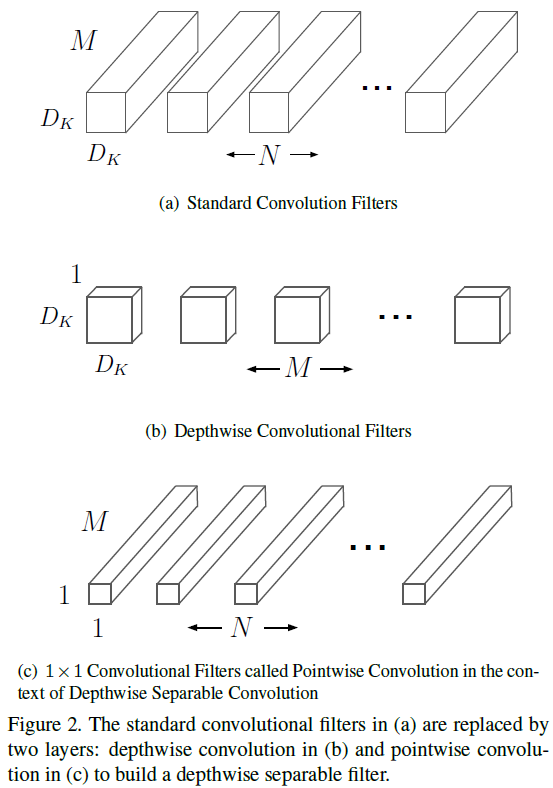
\includegraphics[width=8cm]{images/models/depthwise_separable_conv.png}
    \label{fig:depthwise_separable_conv}
\end{figure}

\subsection{MobileNets}
\begin{figure}[H]
    \centering
    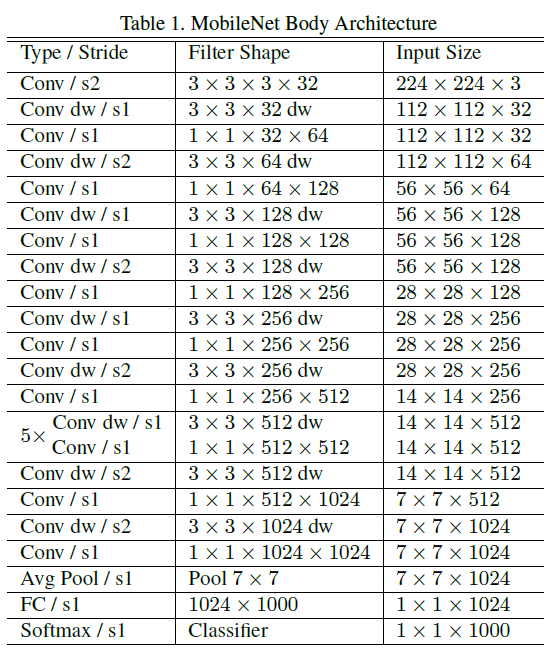
\includegraphics[width=8cm]{images/models/mobilenets.png}
    \label{fig:mobilenets}
\end{figure}

\section{ShuffleNet}
\subsection{Channel Shuffle}
\begin{figure}[H]
    \centering
    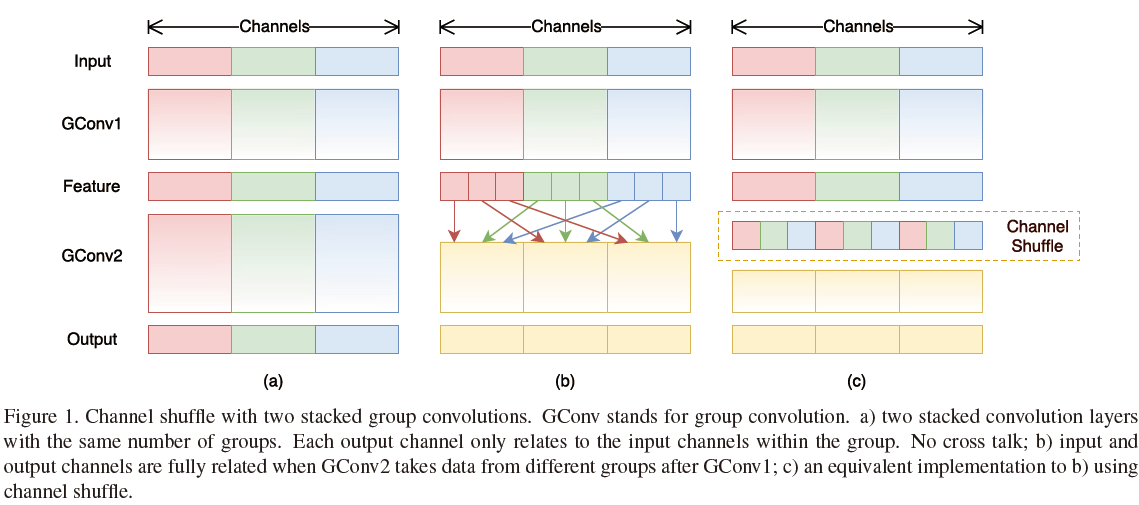
\includegraphics[width=16cm]{images/models/channel_shuffle.png}
    \label{fig:channel_shuffle}
\end{figure}

\subsection{ShuffleNet Unit}
\begin{figure}[H]
    \centering
    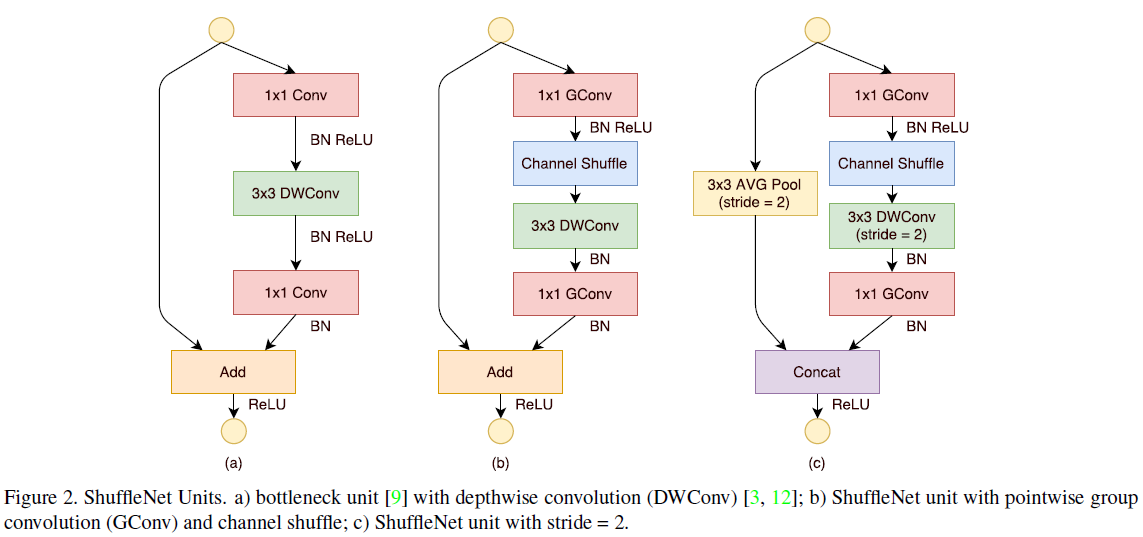
\includegraphics[width=16cm]{images/models/shufflenet_unit.png}
    \label{fig:shufflenet_unit}
\end{figure}

\subsection{ShuffleNet}
\begin{figure}[H]
    \centering
    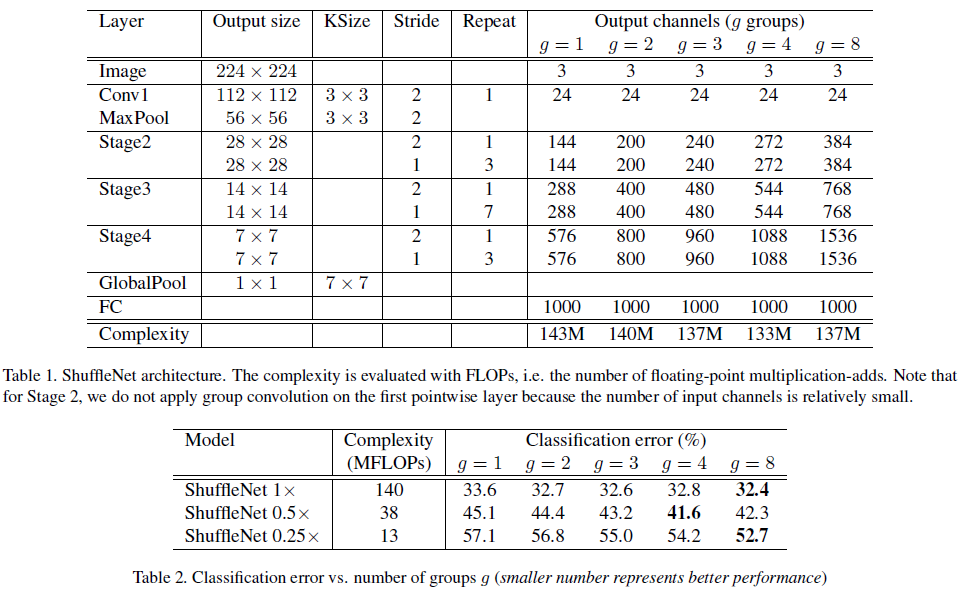
\includegraphics[width=16cm]{images/models/shufflenet.png}
    \label{fig:shufflenet}
\end{figure}

\section{MobileNetv2}

\subsection{Bottleneck residual block}

\begin{figure}[H]
    \centering
    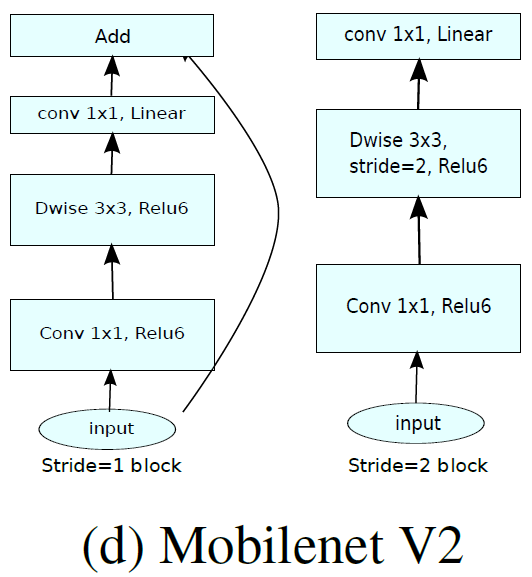
\includegraphics[width=6cm]{images/models/mobilenetv2_block.png}
    \label{fig:mobilenetv2_block}
\end{figure}

\begin{figure}[H]
    \centering
    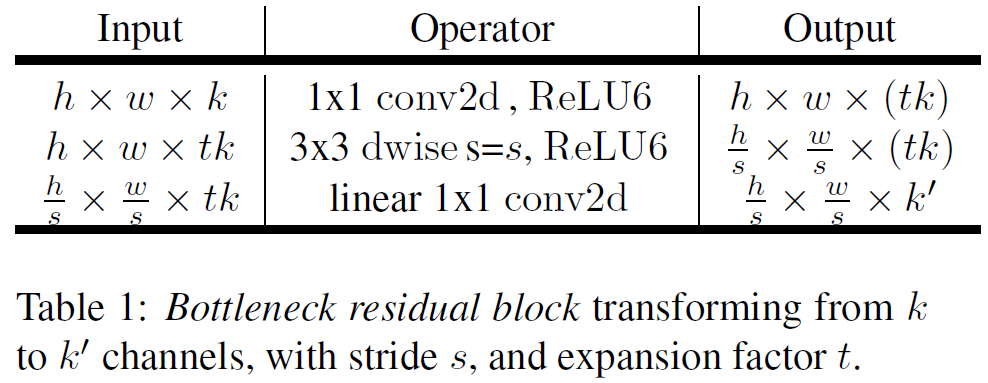
\includegraphics[width=8cm]{images/models/bottleneck_residual_block.png}
    \label{fig:bottleneck_residual_block}
\end{figure}

\subsection{MobileNetv2}
\begin{figure}[H]
    \centering
    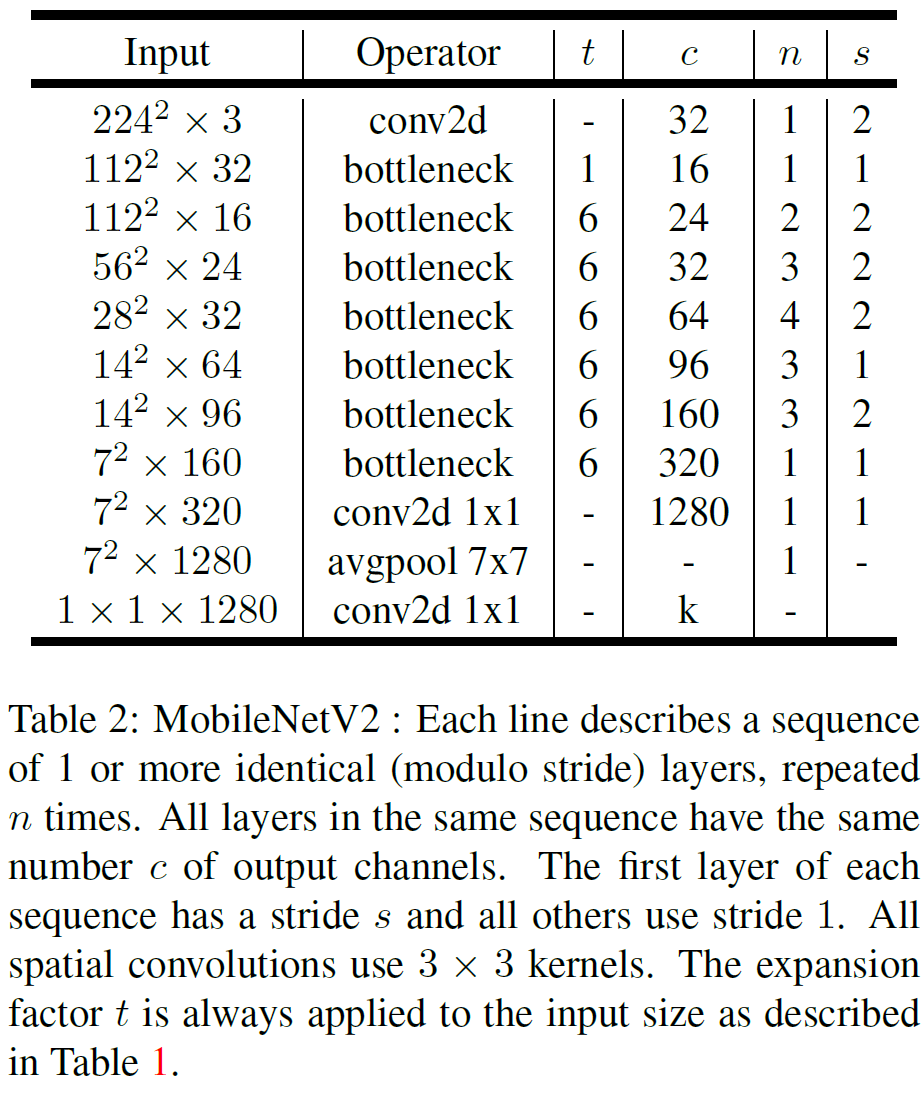
\includegraphics[width=8cm]{images/models/mobilenetv2.png}
    \label{fig:mobilenetv2}
\end{figure}

\section{ShuffleNetv2}
\subsection{ShuffleNetv2 Blocks}
\begin{figure}[H]
    \centering
    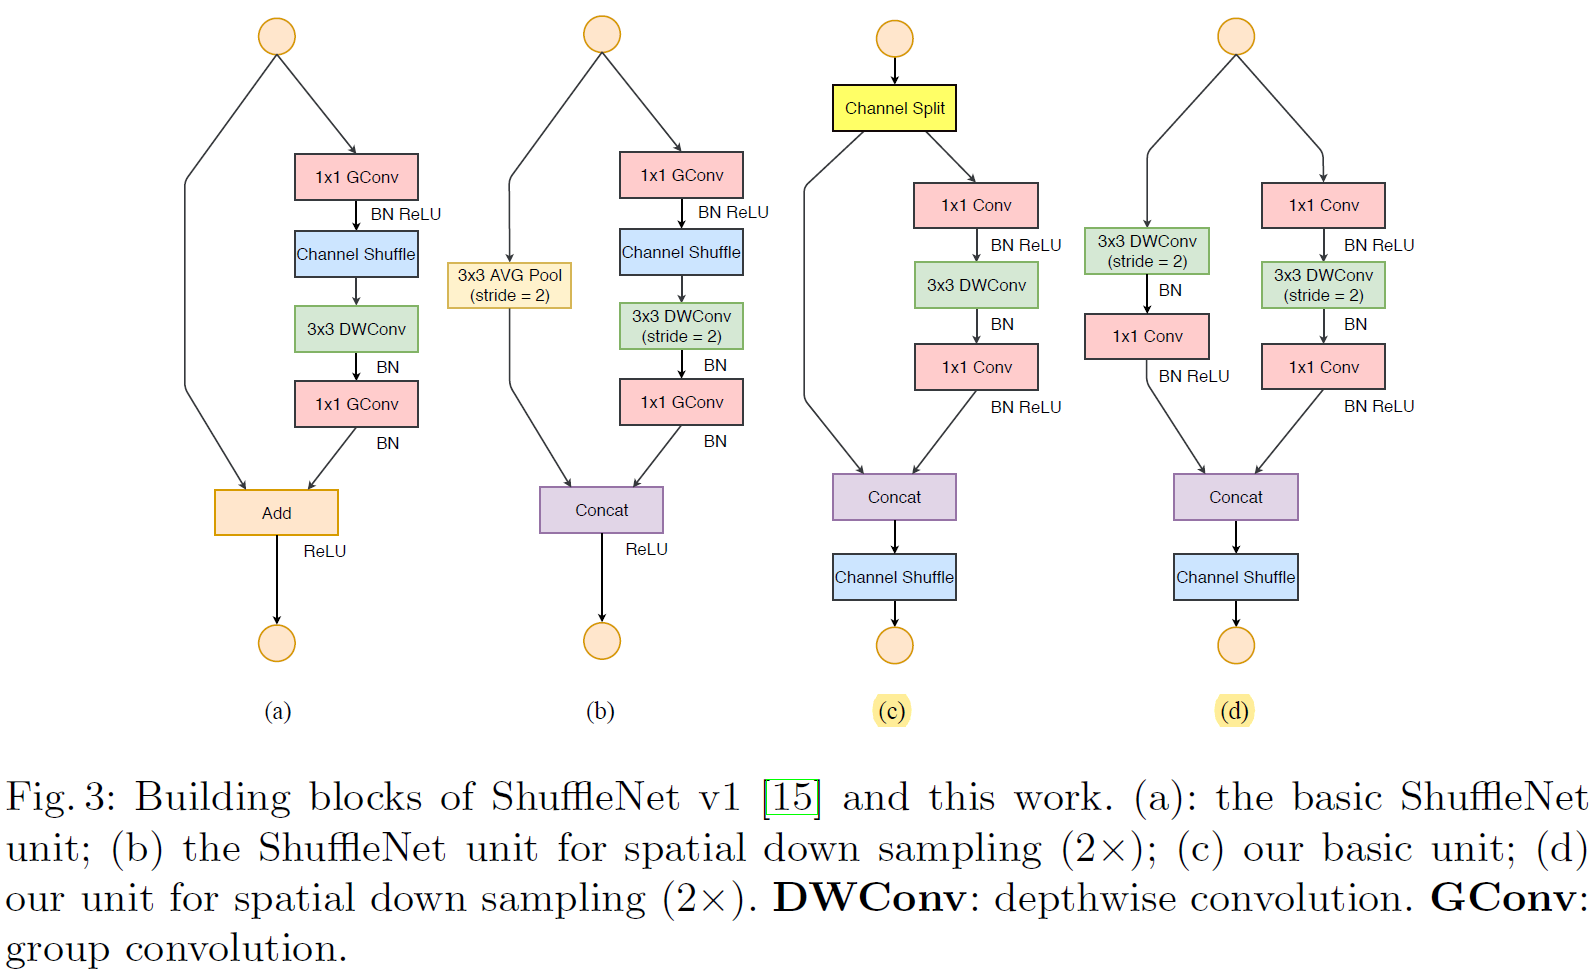
\includegraphics[width=8cm]{images/models/shufflenetv2_block.png}
    \label{fig:shufflenetv2_block}
\end{figure}

\subsection{ShuffleNetv2}
\begin{figure}[H]
    \centering
    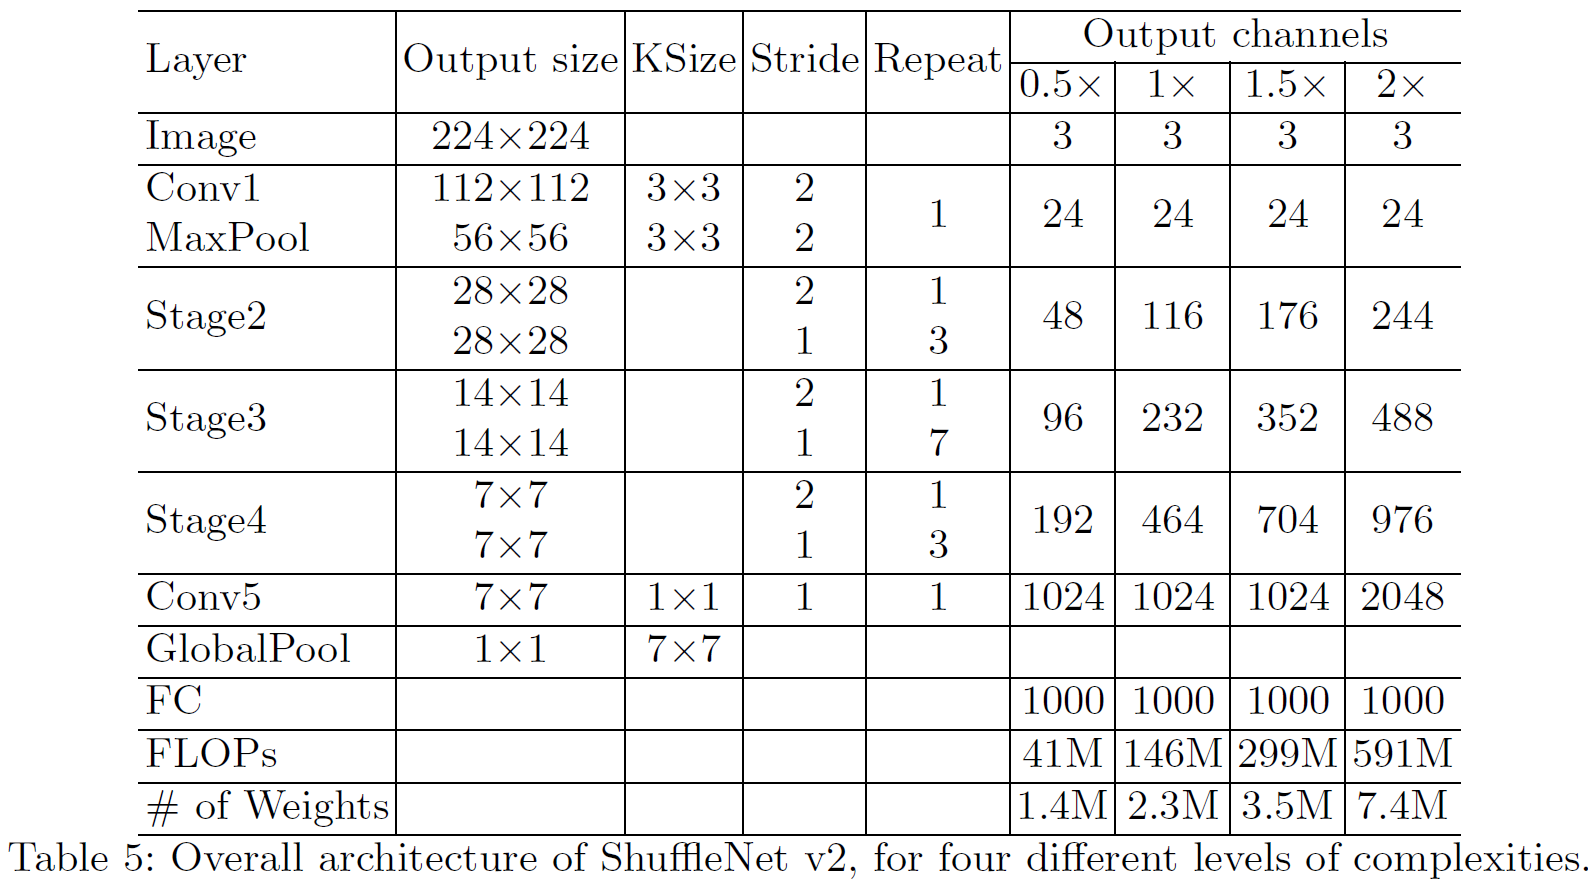
\includegraphics[width=8cm]{images/models/shufflenetv2.png}
    \label{fig:shufflenetv2}
\end{figure}

\subsection{Results}
\begin{figure}[H]
    \centering
    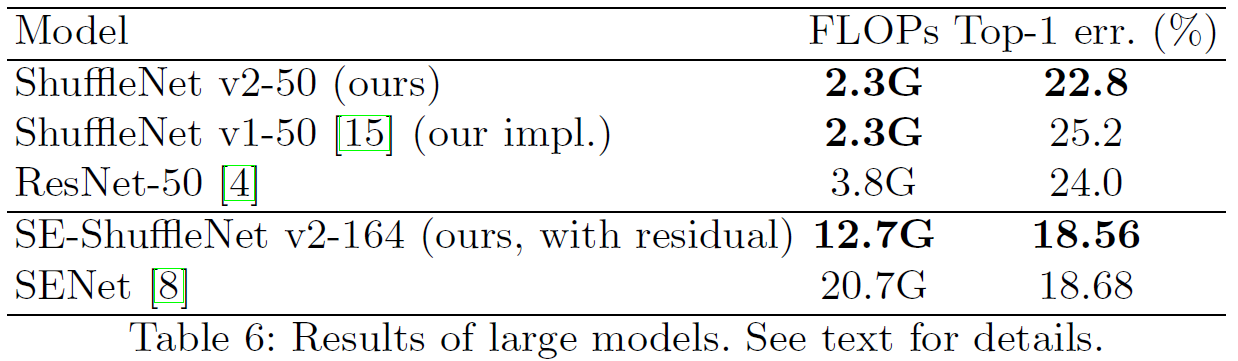
\includegraphics[width=8cm]{images/models/shufflenetv2_res.png}
    \label{fig:shufflenetv2_res}
\end{figure}
\chapter{Skip Connections}

\section{Residual Units}
为了训练deeper model,并解决梯度消失/爆炸以及网络degradation problem,在ResNets\cite{He2016resnet}中提出,如果在shallower model
中添加identity mapping,那么deeper model理应不会有更高的错误率。
\par
Residual unit表示如下:
\begin{equation}
    \begin{split}
        \vy_l &= h(\vx_l) + \mathcal{F}(\vx_l, \mathcal{W}_l) \\
        \vx_{l+1} &= f(\vy_l)
    \end{split}
\end{equation}
In ResNet,$h(\vx_) = \vx_l$ is an identity mapping and $f$ is a ReLU function.
\par
在ResNet中,因为$f$不是identity mapping,所以残差只能ResNet units中学习且信息不能直接传达到后面的层中,
In \cite{He2016identity},希望\textit{propagating information}可以\textit{through theentire network}.
\begin{quotation}
    Our derivations reveal that \textit{if both $h(\vx_l)$ and
$f(\vy_l)$ are identity mappings}, the signal could be \textit{directly}
propagated from one unit to any other units, in both forward and backward passes.\cite{He2016identity}
\end{quotation}

if $f$ is also an identity mapping:
\begin{equation}
    \begin{split}
        \vx_{l+1} = \vx_l + \mathcal{F}(\vx_l, \mW_l)
    \end{split}
\end{equation}
then we will have:
\begin{equation}
    \begin{split}
        \vx_{l+n} &= \vx_{l + n - 1} + \mathcal{F}(\vx_{l + n -1}, \mathcal{W}_{l + n -1}) \\
        &= \vx_{l + n - 2} + \mathcal{F}(\vx_{l + n - 2}, \mathcal{W}_{l + n - 2}) + \mathcal{F}(\vx_{l + n -1}, \mathcal{W}_{l + n -1})\\
        &= \vx_l + \sum_{i=l}^{l+n-1} \mathcal{F}(\vx_i, \mathcal{W}_i)
    \end{split}
\end{equation}
相较于plain network(ignoring BN and ReLU is an identity mapping):
\begin{equation}
    \begin{split}
        \vx_{l+n} &= \prod_{i=l}^{l+n-1} \mW_i \vx_i
    \end{split}
\end{equation}
反向传播过程:
\begin{equation}
    \begin{split}
        \frac{\partial \E}{\partial \vx_l}
        &= \frac{\partial \E}{\partial \vx_{l+n}} \frac{\partial \vx_{l+n}}{\partial \vx_l} \\
        &= \frac{\partial \E}{\partial \vx_{l+n}} \Bigg (1 + \frac{\partial}{\partial \vx_{l}}\sum_{i=l}^{l+n-1} \mathcal{F}(\vx_i, \mathcal{W}_i)\Bigg)
    \end{split}
\end{equation}
可以看出,上式可以分为两部分,$\frac{\partial \E}{\partial \vx_{l+n}}$不经过任何权重信息,可以直接传播到浅层,
只要括号中的第二部分不总是为$-1$,那么\textbf{即使权重任意小也不会发生梯度消失}。

\begin{figure}[H]
    \centering
    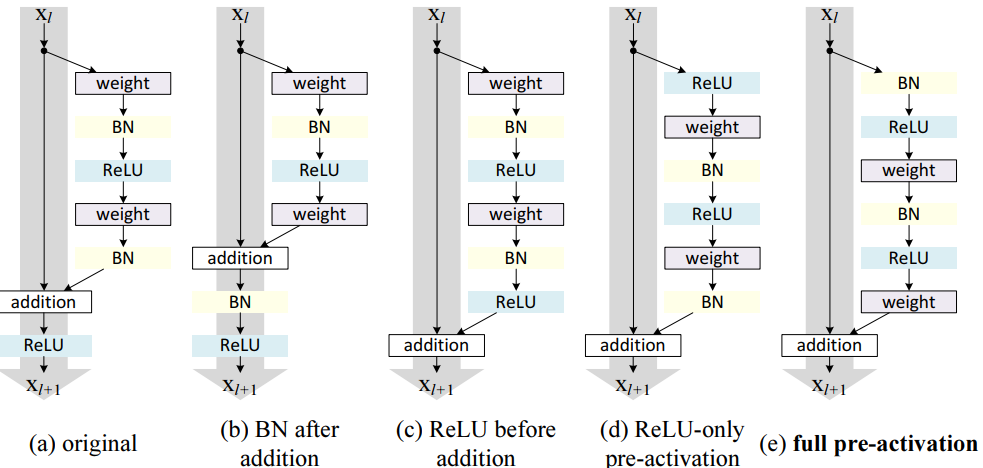
\includegraphics[width=14cm]{images/residual_units.png}
    \caption{Residual Units}
    \label{fig:residual_units}
\end{figure}

以上的分析基于$f$是一个恒等变换,但实际上$f$会影响之前分析的两条信息传播的路径:
\begin{equation}
    \vx_{l+1} = f(\vx_l) + \mathcal{F}(f(\vx_l), \mathcal{W}_l)
\end{equation}
因此,在\cite{He2016identity}提出了新的Residual unit结构pre-activation,等式变为
\begin{equation}
    \vx_{l+1} = \vx_l + \mathcal{F}(\hat f(\vx_l), \mathcal{W}_l)
\end{equation}

\section{The Shattered Gradients Problem}
\begin{quotation}
    A previously unnoticed difficulty with gradients in deep rectifier networks that orthogonal
    to vanishing and exploding gradients. The shattering gradients problem is that, as depth increases,
    \textbf{gradients in standard feedforward networks increasingly resemble white noise}\cite{Balduzzi2017}.
\end{quotation}
\begin{itemize}
    \item Gradients of shallow networks resemble brown noise(布朗噪声).
    \item Gradients of deep networks resemble white noise(白噪声).
    \item Training is difficult when gradients behave like white noise.
    \item Gradients of deep resnets lie in between brown and white noise.
\end{itemize}

在标准前馈神经网络中,神经元相关性按指数级减少($\frac{1}{2^L}$),同时,梯度的空间结构也随着深度增加被逐渐消除。
使用BatchNorm的ResNets中梯度相关系减少的速度从指数级减少到亚线性级($\frac{1}{\sqrt(L)}$),极大的保留梯度的空间结构。

\begin{figure}[H]
    \centering
    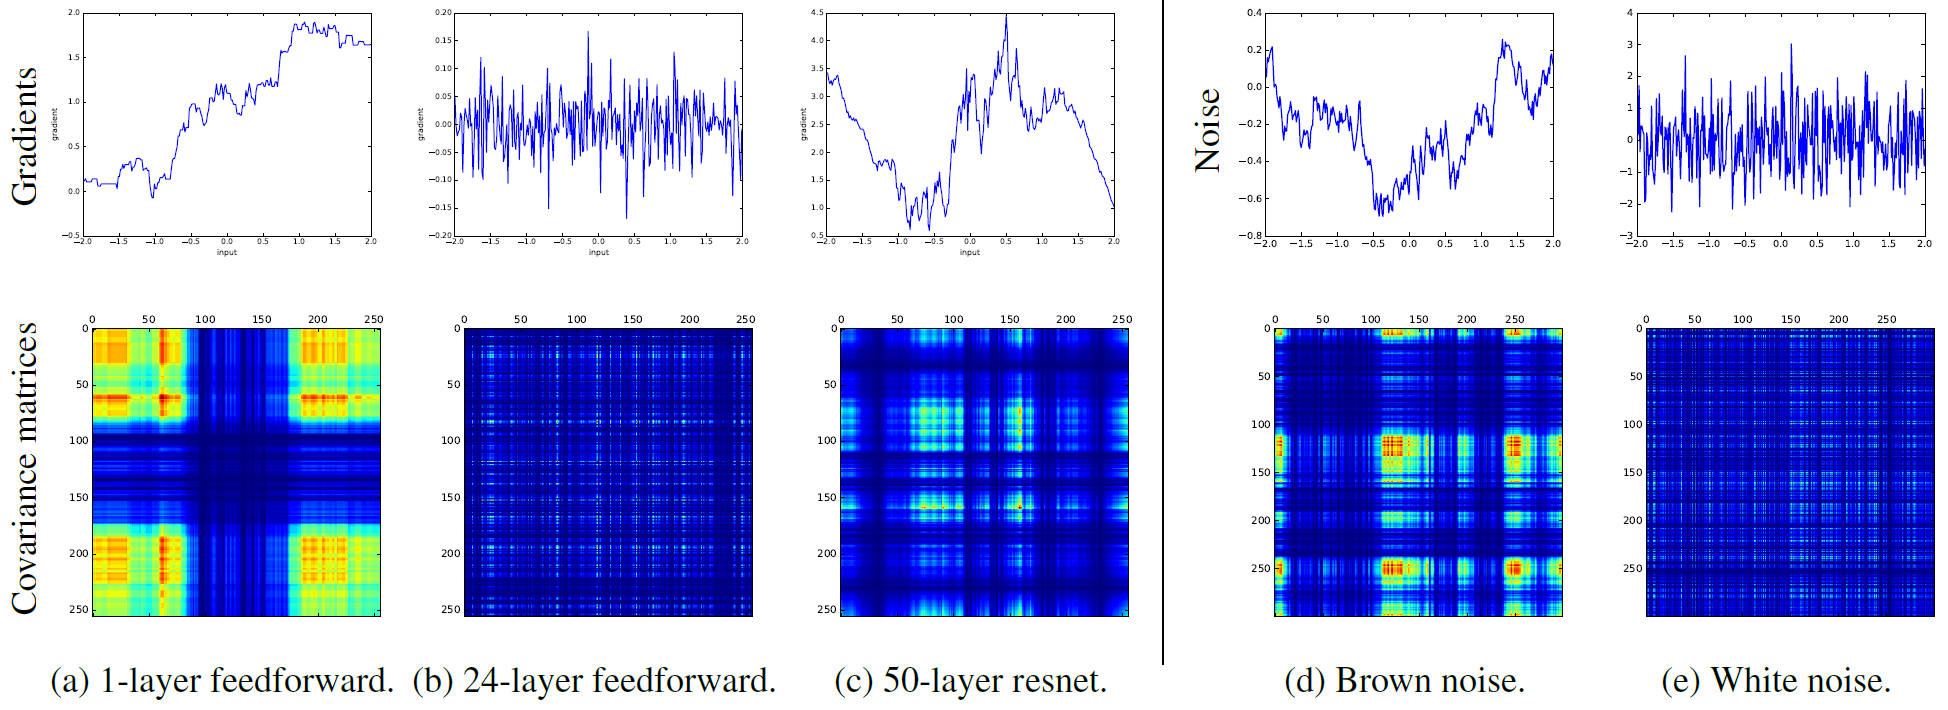
\includegraphics[width=14cm]{images/brown_white_noise.png}
    \caption{The shattered Gradients Problem}
    \label{fig:brown_white_noise}
\end{figure}


\section{DenseNet}
\begin{figure}[H]
    \centering
    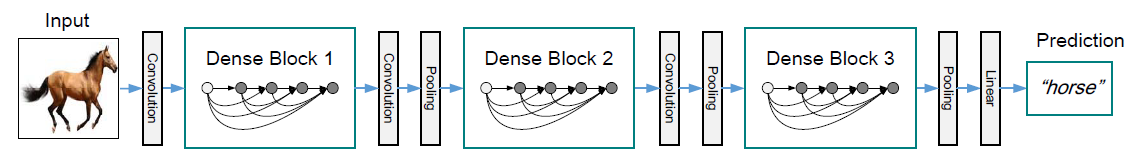
\includegraphics[width=14cm]{images/densenet.png}
    \caption{DenseNet}
    \label{fig:densenet}
\end{figure}

\section{FCN}
\begin{figure}[H]
    \centering
    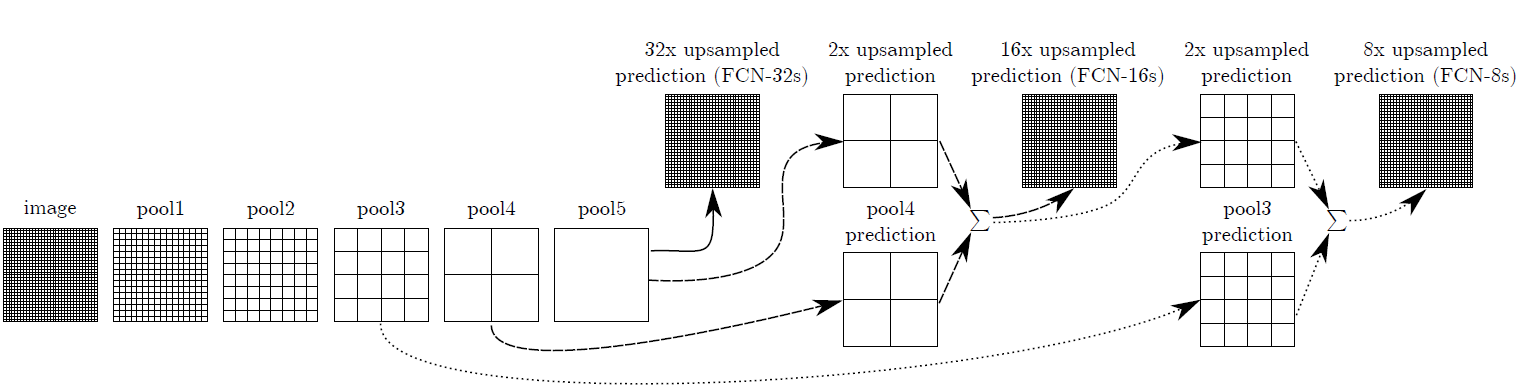
\includegraphics[width=14cm]{images/fcns.png}
    \caption{FCN}
    \label{fig:fcn}
\end{figure}

\section{UNet family}
\subsection{U-Net}

\subsubsection{Architecture}
\begin{figure}[H]
    \centering
    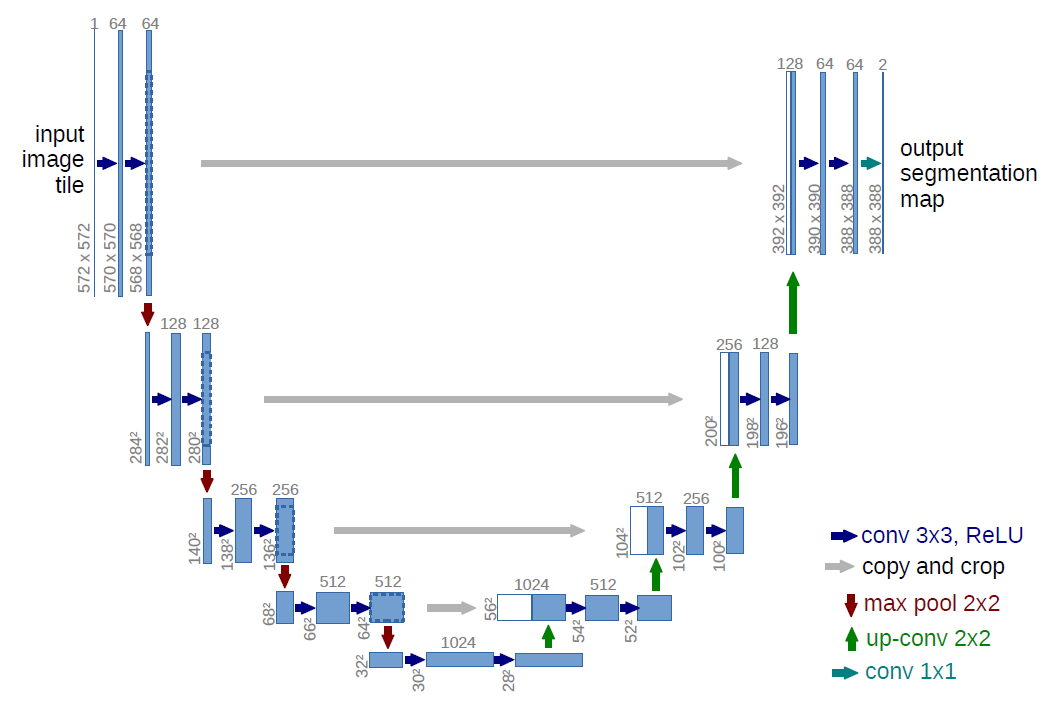
\includegraphics[width=10cm]{images/unet.png}
    \caption{UNet}
    \label{fig:unet}
\end{figure}
UNet\cite{UNet2015}: The architecture consists of a \textbf{contracting path} to capture
context and a symmetric \textbf{expanding path} that enables precise localization.

[offical implementation]\url{http://lmb.informatik.uni-freiburg.de/people/ronneber/u-net}

\subsubsection{Metrics}

\subsection{VNet}

\subsubsection{Dice coeffcient}
\[
dice = \frac{2|X \cap Y |}{|X| + |Y|}
\]


\subsection{UNet 2+}

\begin{figure}[H]
    \centering
    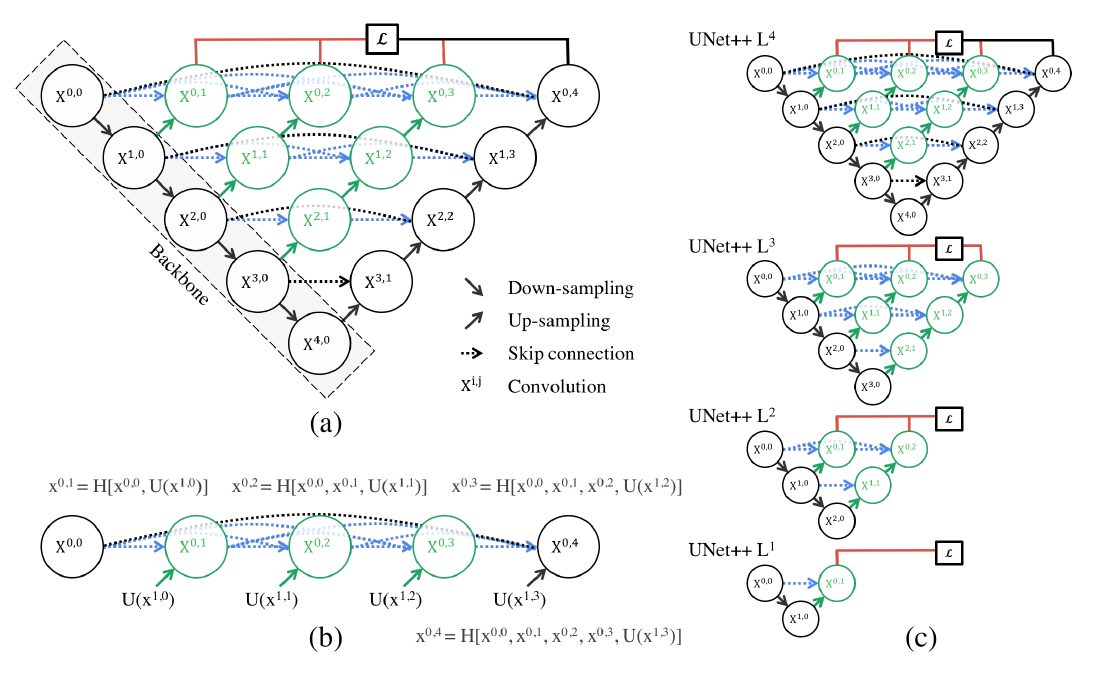
\includegraphics[width=14cm]{images/unet2+.png}
    \caption{UNet 2+}
    \label{fig:unet2p}
\end{figure}

多深合适?降采样对分割网络到底是不是必须的?
不一定要降到第四次才上采样,使用浅层和深层的特征。

\subsection{UNet 3+}

\begin{figure}[H]
    \centering
    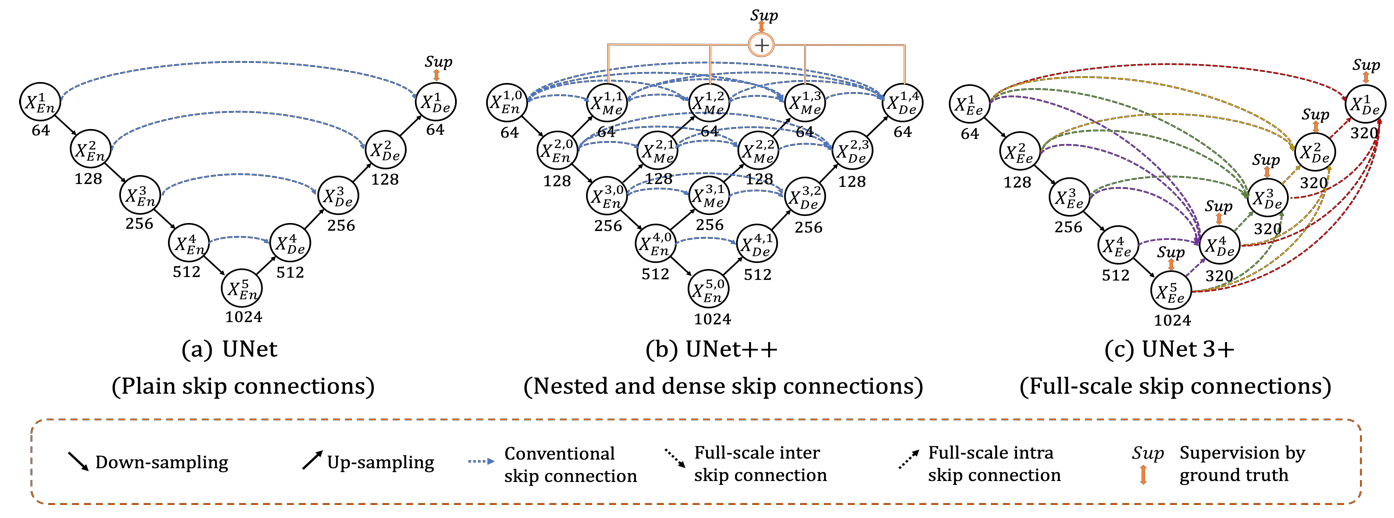
\includegraphics[width=14cm]{images/unet3+.png}
    \caption{UNet 3+}
    \label{fig:unet3p}
\end{figure}
都缺乏从全尺度探索足够信息的能力,未能明确了解器官的位置和边界。UNet 3+中的每一个解码器层都融合了来自编码器中的小尺度和同尺度的特征图,
以及来自解码器的大尺度的特征图,这些特征图捕获了全尺度下的细粒度语义和粗粒度语义。

\chapter{Semantic Segmentation}

\section{FCN - Fully Convolutional Network}

\subsection{Metrics}
Let $p_{ij}$ be the number of pixels of class $i$ predicted to belong to class $j$.

\subsubsection{Pixel accuracy}

\[
    PA = \frac{\sum\limits_{i=0}^k p_{ii}}{\sum\limits_{i=0}^k \sum\limits_{j=0}^k p_{ij}}
\]

\subsubsection{Mean accuraccy}

\[
    MPA = \frac{1}{k + 1} \sum\limits_{i=0}^k \frac{p_{ii}}{\sum\limits_{j=0}^k p_{ij}}
\]

\subsubsection{Mean IoU}

\[
    MIoU = \frac{1}{k + 1} \sum_{i=0}^k \frac{p_{ii}}{\sum\limits_{j=0}^k p_{ij} + \sum\limits_{j=0}^k p_{ji} - p_{ii}}
\]

\subsubsection{f-score}

\[
    f-score = (1 + \beta ^2) \frac{precision \cdot recall}{\beta^2 \cdot precision + recall}
\]

\subsubsection{dice coeffience}
\[
    dice-coeff = f_{1}-score
\]
\chapter{Autoencoder}

\begin{figure}[H]
    \centering
    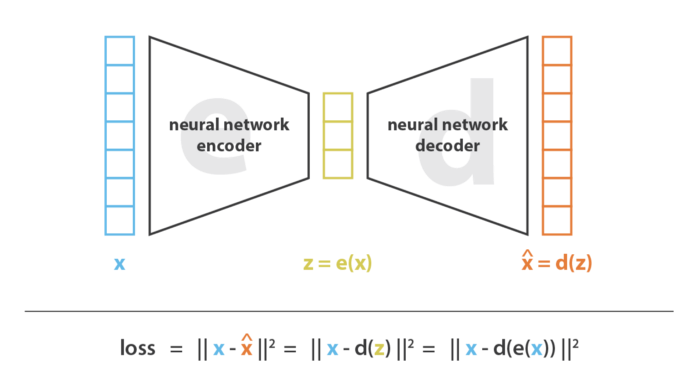
\includegraphics[width=10cm]{images/ae.png}
    \caption{Autoencoder}
    \label{fig:autoencoder}
\end{figure}
\section{linear autoencoder VS PCA}
\section{欠完备自编码器}
编码维度小于输入维度。学习欠完备的表示将强制自编码器捕捉训练数据中最显著的特征(降维->特征)。

\section{正则自编码器}
如果隐藏层的编码的维度允许与输入相等,或隐藏编码维数大于输入的过完备的情况下,会学习将输入复制到输出,而学不到任何有关数据分布的的有用信息。
正则自编码器使用的损失函数可以鼓励模型学习其他特性(除了将输入复制到输出),而不必限制使用浅层的编码器和解码器以及小的编码维度来限制模型的容量。这些
特性包括稀疏表示、表示的小导数以及对噪声或输入缺失的鲁棒性,即使模型容量大到足以学习一个无意义的恒等函数,非线性
且过完备的正则自编码器仍然能够从数据中学到一些关于数据分布的有用信息。

\subsection{稀疏自编码器}
\begin{equation}
    L(\vx, g(f(\vx))) + \Omega (h)
\end{equation}
\subsection{DAE - Denoising Autoencoder}
\begin{equation}
    L(\vx, g(f(\tilde{\vx})))
\end{equation}
\subsection{CAE - Contractive Autoencoder}
\begin{equation}
    \begin{split}
        L(\vx, g(f(\vx))) + \Omega(\vh, \vx) \\
        \Omega(\vh, \vx) = \lambda \sum_i \| \nabla_x h_i \|^2
    \end{split}
\end{equation}


\chapter{Generative Adversarial Nets}

\section{GAN}

\section{CGAN}

\bibliographystyle{plain}
\bibliography{references}
\end{document}